% =========================================================
%
%  ANNA UNIVERSITY B.E. / B.TECH. PROJECT REPORT TEMPLATE
%
%  A reusable LaTeX template following the official
%  Anna University (Chennai 600 025) formatting guidelines
%  for undergraduate project reports.
%
%  Compiler:   XeLaTeX (required for Times New Roman font)
%  Created:    November 2026
%  Version:    1.0
%
% =========================================================
%
%  HOW TO COMPILE (Overleaf):
%    1. Upload this entire folder to Overleaf as a new project.
%    2. Go to Menu → Compiler → Select "XeLaTeX".
%    3. Click "Recompile" (or Ctrl+Enter).
%    4. Compile TWICE for Table of Contents and references
%       to update correctly.
%
%  HOW TO COMPILE (Local):
%    xelatex main.tex
%    bibtex main
%    xelatex main.tex
%    xelatex main.tex
%
% =========================================================
%
%  QUICK START — To customize this template for your project:
%    1. Edit config/metadata.tex — fill in your project details.
%    2. Place your logo files in the figures/ folder.
%    3. Edit frontmatter/abstract.tex — write your abstract.
%    4. Edit frontmatter/acknowledgement.tex — update names.
%    5. Edit chapters/ files — write your chapter content.
%    6. Edit bibliography.bib — add your references.
%    7. Edit frontmatter/list_of_abbreviations.tex — add yours.
%    8. Compile and review.
%
% =========================================================

% ---------------------------------------------------------
% DOCUMENT CLASS
% ---------------------------------------------------------
% 'report' class: provides chapter-level organization.
% '12pt': base font size. We override this to 14pt in
%   config/formatting.tex using \renewcommand{\normalsize}.
% 'a4paper': A4 page size (mandatory per AU guidelines).
% 'oneside': single-sided printing (standard for project reports).
%
% NOTE: We use 12pt as the class option because LaTeX's report
% class does not natively support 14pt. The actual 14pt size is
% set in formatting.tex via \fontsize{14}{21}\selectfont.
% DO NOT CHANGE to 10pt or 11pt.
% ---------------------------------------------------------
\documentclass[12pt, a4paper, oneside]{report}

% ---------------------------------------------------------
% LOAD CONFIGURATION FILES
% ---------------------------------------------------------
% These files must be loaded in this exact order:
%   1. metadata.tex — project-specific information
%   2. packages.tex — all package imports
%   3. formatting.tex — page layout, fonts, spacing, headings
%   4. commands.tex — custom commands and shortcuts
% ---------------------------------------------------------

% Step 1: Project metadata (must be loaded FIRST because
% other files reference these commands)
% =========================================================
% PROJECT METADATA — SINGLE SOURCE OF TRUTH
% =========================================================

% ---------------------------------------------------------
% PROJECT INFORMATION
% ---------------------------------------------------------
\newcommand{\ProjectTitle}{QUERYPILOT: AN UNCERTAINTY-AWARE, SELF-ADAPTIVE QUERY OPTIMIZATION FRAMEWORK FOR DYNAMIC DATABASE WORKLOADS}
\newcommand{\ProjectPhase}{}

% ---------------------------------------------------------
% STUDENT INFORMATION
% ---------------------------------------------------------
\newcommand{\StudentOneName}{NITISH M}
\newcommand{\StudentOneRegNo}{[312423104156]}

\newcommand{\StudentTwoName}{PADMESH V A}
\newcommand{\StudentTwoRegNo}{[312423104158]}

% ---------------------------------------------------------
% DEGREE AND DEPARTMENT INFORMATION
% ---------------------------------------------------------
\newcommand{\DegreeName}{BACHELOR OF ENGINEERING}
\newcommand{\BranchName}{COMPUTER SCIENCE AND ENGINEERING}
\newcommand{\DepartmentName}{Computer Science and Engineering}
\newcommand{\Semester}{VIII}

% ---------------------------------------------------------
% COLLEGE INFORMATION
% ---------------------------------------------------------
\newcommand{\CollegeName}{St. Joseph's Institute of Technology}
\newcommand{\CollegeLocation}{Chennai}
\newcommand{\CollegeAutonomous}{(An Autonomous Institution)}
\newcommand{\CollegeAddress}{Old Mamallapuram Road, Chennai -- 600 119.}
\newcommand{\UniversityName}{ANNA UNIVERSITY :: CHENNAI 600025}

% ---------------------------------------------------------
% GUIDE / SUPERVISOR INFORMATION
% ---------------------------------------------------------
\newcommand{\GuideName}{Dr. V. Sabaresan}
\newcommand{\GuideDesignation}{Assistant Professor}
\newcommand{\GuideQualification}{M.E., Ph.D.}

% ---------------------------------------------------------
% HEAD OF DEPARTMENT INFORMATION
% ---------------------------------------------------------
\newcommand{\HODName}{Dr. J. Dafni Rose}
\newcommand{\HODDesignation}{Professor \& Head}
\newcommand{\HODQualification}{M.E., Ph.D.}

% ---------------------------------------------------------
% COLLEGE MANAGEMENT
% ---------------------------------------------------------
\newcommand{\ChairmanName}{Dr. B. Babu Manoharan}
\newcommand{\ChairmanQualification}{M.A., M.B.A., Ph.D.}

\newcommand{\ManagingDirectorName}{Mr. B. Sashi Sekar}
\newcommand{\ManagingDirectorQualification}{M.Sc.}

\newcommand{\ExecutiveDirectorName}{Mrs. S. Jessie Priya}
\newcommand{\ExecutiveDirectorQualification}{M.Com.}

\newcommand{\PrincipalName}{Dr. R. Priscilla}
\newcommand{\PrincipalQualification}{M.E., Ph.D.}

% ---------------------------------------------------------
% SUBMISSION DETAILS
% ---------------------------------------------------------
\newcommand{\SubmissionMonth}{NOVEMBER}
\newcommand{\SubmissionYear}{2026}
\newcommand{\SubmissionDate}{\SubmissionMonth{} \SubmissionYear}
\newcommand{\AcademicYear}{2026--2027}

% ---------------------------------------------------------
% LOGO FILE PATHS
% ---------------------------------------------------------
\newcommand{\CollegeLogoFile}{figures/st josephs.png}
\newcommand{\UniversityLogoFile}{figures/Anna university.png}


% Step 2: Package imports
% =========================================================
% PACKAGE DECLARATIONS
% =========================================================
% All LaTeX packages required by this template are loaded here.
% Each package includes a comment explaining why it is needed.
%
% IMPORTANT: Do not remove packages unless you are sure they
% are not used anywhere in the template. Adding new packages
% here is safe — just place them at the end of this file.
% =========================================================

% ---------------------------------------------------------
% FONT SUPPORT (XeLaTeX)
% ---------------------------------------------------------
% fontspec: Required for XeLaTeX to use system fonts like
% Times New Roman. This is the recommended approach for
% matching the Anna University requirement exactly.
% DO NOT REMOVE — the entire template depends on this.
\usepackage{fontspec}

% ---------------------------------------------------------
% LANGUAGE AND ENCODING
% ---------------------------------------------------------
% For English-only documents with XeLaTeX, explicit language
% setup is not required. If you need multilingual support,
% uncomment the two lines below:
% \usepackage{polyglossia}
% \setmainlanguage{english}

% ---------------------------------------------------------
% PAGE LAYOUT
% ---------------------------------------------------------
% geometry: Controls page dimensions and margins.
% The margin values here implement the official Anna University
% requirements. See FORMAT_RULES.md, Section 2.
\usepackage{geometry}

% ---------------------------------------------------------
% LINE SPACING
% ---------------------------------------------------------
% setspace: Provides \onehalfspacing, \doublespacing,
% and \singlespacing commands for controlling line spacing
% throughout the document.
\usepackage{setspace}

% ---------------------------------------------------------
% HEADERS AND FOOTERS
% ---------------------------------------------------------
% fancyhdr: Customizes headers and footers.
% Used to place page numbers at the center bottom.
\usepackage{fancyhdr}

% ---------------------------------------------------------
% TABLE OF CONTENTS FORMATTING
% ---------------------------------------------------------
% tocloft: Customizes the Table of Contents, List of Figures,
% and List of Tables formatting (fonts, spacing, leader dots).
\usepackage[titles]{tocloft}

% ---------------------------------------------------------
% CHAPTER AND SECTION HEADING STYLES
% ---------------------------------------------------------
% titlesec: Customizes the formatting of chapter titles,
% section headings, and subsection headings to match the
% Anna University format (centered chapter titles, etc.).
\usepackage{titlesec}

% ---------------------------------------------------------
% GRAPHICS
% ---------------------------------------------------------
% graphicx: Required for inserting images (\includegraphics).
% Used for logos, diagrams, screenshots, and figures.
\usepackage{graphicx}

% ---------------------------------------------------------
% COLORS (optional, for hyperlinks)
% ---------------------------------------------------------
\usepackage{xcolor}

% ---------------------------------------------------------
% TABLES
% ---------------------------------------------------------
% booktabs: Provides professional-quality table rules
% (\toprule, \midrule, \bottomrule) instead of ugly \hline.
\usepackage{booktabs}

% array: Extended column definitions for tables.
\usepackage{array}

% longtable: For tables that span multiple pages.
\usepackage{longtable}

% tabularx: Tables with auto-adjusting column widths.
\usepackage{tabularx}

% multirow: Allows cells to span multiple rows in tables.
\usepackage{multirow}

% ---------------------------------------------------------
% CAPTIONS
% ---------------------------------------------------------
% caption: Customizes figure and table caption formatting.
% Used to make captions bold and properly sized.
\usepackage{caption}

% ---------------------------------------------------------
% MATHEMATICAL TYPESETTING
% ---------------------------------------------------------
% amsmath: Standard package for mathematical equations,
% aligned environments, and math symbols.
\usepackage{amsmath}

% amssymb: Additional math symbols.
\usepackage{amssymb}

% ---------------------------------------------------------
% CODE LISTINGS
% ---------------------------------------------------------
% listings: For typesetting source code with syntax highlighting.
% Used in Chapter 6 (Results and Coding) for sample code.
\usepackage{listings}

% ---------------------------------------------------------
% HYPERLINKS AND CROSS-REFERENCES
% ---------------------------------------------------------
% hyperref: Makes cross-references, citations, TOC entries,
% and URLs clickable in the PDF. Colors are set to black
% for print compatibility.
\usepackage[hidelinks]{hyperref}

% ---------------------------------------------------------
% BIBLIOGRAPHY
% ---------------------------------------------------------
% natbib: Flexible bibliography support with author-year
% and numbered citation styles. Used with plainnat style
% for alphabetical ordering as required by AU guidelines.
\usepackage[numbers,sort&compress]{natbib}

% ---------------------------------------------------------
% APPENDIX SUPPORT
% ---------------------------------------------------------
% appendix: Provides additional control over appendix formatting.
\usepackage[toc,page]{appendix}

% ---------------------------------------------------------
% LIST CUSTOMIZATION
% ---------------------------------------------------------
% enumitem: Customizes itemize, enumerate, and description lists.
\usepackage{enumitem}

% ---------------------------------------------------------
% PDF METADATA
% ---------------------------------------------------------
% This sets the PDF document properties (visible in PDF readers).
% The values are pulled from metadata.tex commands.
\AtBeginDocument{%
  \hypersetup{
    pdftitle={\ProjectTitle},
    pdfauthor={\StudentOneName},
    pdfsubject={B.E. Project Report},
    pdfkeywords={Anna University, Project Report, \BranchName},
  }%
}


% Step 3: Formatting rules (margins, fonts, spacing, etc.)
% =========================================================
% FORMATTING CONFIGURATION
% =========================================================
% This file implements ALL the visual formatting rules from
% the Anna University guidelines. Each setting references
% the corresponding rule in FORMAT_RULES.md.
%
% IMPORTANT: Values marked "DO NOT CHANGE" are mandatory
% per official guidelines. Values marked "CUSTOMIZABLE"
% can be safely adjusted.
% =========================================================

% ---------------------------------------------------------
% PAGE MARGINS
% ---------------------------------------------------------
% Source: WhatsApp Image (margin specs), FORMAT_RULES.md §2
%
% Official requirements (ranges):
%   Top:    30–35 mm    → using 32 mm
%   Bottom: 25–30 mm    → using 27 mm
%   Left:   35–40 mm    → using 37 mm (extra for binding)
%   Right:  20–25 mm    → using 22 mm
%
% DO NOT CHANGE these below the minimum values.
% CUSTOMIZABLE within the stated ranges only.
% ---------------------------------------------------------
\geometry{
  a4paper,
  top=32mm,
  bottom=27mm,
  left=37mm,
  right=22mm,
}

% ---------------------------------------------------------
% FONT CONFIGURATION
% ---------------------------------------------------------
% Source: UG_REPORT_FORMAT.pdf §4, FORMAT_RULES.md §3
%
% Official requirement: Times New Roman for all text.
% DO NOT CHANGE the font family.
%
% NOTE FOR OVERLEAF: XeLaTeX on Overleaf has Times New Roman
% available as a system font. If compilation fails, try
% using "TeX Gyre Termes" as the fallback — it is metrically
% identical to Times New Roman and always available.
% ---------------------------------------------------------
\setmainfont{Times New Roman}[
  Ligatures=TeX,
]
% Fallback if Times New Roman is unavailable:
% \setmainfont{TeX Gyre Termes}[Ligatures=TeX]

% ---------------------------------------------------------
% BASE FONT SIZE
% ---------------------------------------------------------
% Source: UG_REPORT_FORMAT.pdf §4 — "Font size 14"
%
% The document class is set to 12pt as the base. We then
% globally scale to 14pt using \fontsize. The extsize classes
% don't work well with XeLaTeX fontspec, so this approach
% is more reliable.
%
% 14pt font with 1.5 line spacing = 14 × 1.5 = 21pt leading.
% The setspace package handles this more precisely.
% DO NOT CHANGE.
% ---------------------------------------------------------
\renewcommand{\normalsize}{\fontsize{14}{21}\selectfont}
\normalsize

% ---------------------------------------------------------
% LINE SPACING
% ---------------------------------------------------------
% Source: UG_REPORT_FORMAT.pdf §4, FORMAT_RULES.md §4
%
% Default spacing for general text: 1.5 spacing.
% Specific sections override this (abstract=double,
% references=single). Those overrides are applied locally
% in their respective .tex files.
% DO NOT CHANGE.
% ---------------------------------------------------------
\onehalfspacing

% ---------------------------------------------------------
% PARAGRAPH FORMATTING
% ---------------------------------------------------------
% Source: batch_86.pdf (observed)
%
% Paragraph indentation: ~1.27 cm (standard 0.5 inch)
% Paragraph spacing: minimal (handled by line spacing)
% Text alignment: justified
%
% CUSTOMIZABLE: parindent can be adjusted if your department
% prefers a different indentation.
% ---------------------------------------------------------
\setlength{\parindent}{1.27cm}
\setlength{\parskip}{0pt}

% ---------------------------------------------------------
% PAGE NUMBERING AND HEADERS/FOOTERS
% ---------------------------------------------------------
% Source: batch_86.pdf (observed), FORMAT_RULES.md §5
%
% Page numbers: centered at the bottom of the page.
% No running headers or footers.
% Front matter uses Roman numerals; main matter uses Arabic.
% DO NOT CHANGE the number style or position.
% ---------------------------------------------------------
\pagestyle{fancy}
\fancyhf{}
\fancyfoot[C]{\thepage}
\renewcommand{\headrulewidth}{0pt}
\renewcommand{\footrulewidth}{0pt}

% Also apply to plain style (used on chapter opening pages)
\fancypagestyle{plain}{
  \fancyhf{}
  \fancyfoot[C]{\thepage}
  \renewcommand{\headrulewidth}{0pt}
  \renewcommand{\footrulewidth}{0pt}
}

% ---------------------------------------------------------
% CHAPTER HEADING FORMAT
% ---------------------------------------------------------
% Source: batch_86.pdf (observed), FORMAT_RULES.md §7
%
% Chapter headings are centered with:
%   Line 1: "CHAPTER X" (bold, 16pt)
%   Line 2: "CHAPTER TITLE" (bold, 16pt)
%
% There is vertical space before and after the heading block.
% DO NOT CHANGE the centering or bold style.
% CUSTOMIZABLE: vertical spacing values.
% ---------------------------------------------------------
\titleformat{\chapter}[display]
  {\normalfont\fontsize{16}{24}\bfseries\centering}
  {CHAPTER \thechapter}
  {0pt}
  {\MakeUppercase}
\titlespacing*{\chapter}{0pt}{-20pt}{30pt}

% ---------------------------------------------------------
% SECTION HEADING FORMAT
% ---------------------------------------------------------
% Source: batch_86.pdf (observed), FORMAT_RULES.md §7
%
% Section headings: left-aligned, bold.
% Example: "1.1 OVERVIEW"
% Font size: same as body text (14pt), bold.
%
% NOTE: Write section titles in ALL CAPS in your source files
% (e.g., \section{OVERVIEW}). This ensures both the body
% heading and the TOC entry are correctly uppercased.
% ---------------------------------------------------------
\titleformat{\section}
  {\normalfont\fontsize{14}{21}\bfseries}
  {\thesection}{1em}{}
\titlespacing*{\section}{0pt}{18pt}{12pt}

% ---------------------------------------------------------
% SUBSECTION HEADING FORMAT
% ---------------------------------------------------------
% Source: batch_86.pdf (observed)
%
% Subsection headings: left-aligned, bold.
% Example: "3.1.1 Use Case Diagram of Threat Detection"
% Font size: same as body text (14pt), bold.
% NOT uppercased (title case is used in the sample report).
% ---------------------------------------------------------
\titleformat{\subsection}
  {\normalfont\fontsize{14}{21}\bfseries}
  {\thesubsection}{1em}{}
\titlespacing*{\subsection}{0pt}{14pt}{10pt}

% ---------------------------------------------------------
% SUBSUBSECTION HEADING FORMAT
% ---------------------------------------------------------
\titleformat{\subsubsection}
  {\normalfont\fontsize{14}{21}\bfseries}
  {\thesubsubsection}{1em}{}
\titlespacing*{\subsubsection}{0pt}{12pt}{8pt}

% ---------------------------------------------------------
% TABLE OF CONTENTS FORMATTING
% ---------------------------------------------------------
% Source: UG_REPORT_FORMAT.pdf §3.4, Appendix 3
%
% TOC header columns: CHAPTER NO. | TITLE | PAGE NO.
% Entries should be in CAPITAL LETTERS.
% 1.5 line spacing.
% Leader dots connect title to page number.
% ---------------------------------------------------------

% Rename the TOC title
\renewcommand{\contentsname}{TABLE OF CONTENTS}

% Chapter entries in TOC: bold
\renewcommand{\cftchapfont}{\bfseries}
\renewcommand{\cftchappagefont}{\bfseries}
\renewcommand{\cftchapleader}{\cftdotfill{\cftdotsep}}

% Section entries in TOC
\renewcommand{\cftsecfont}{\normalfont}
\renewcommand{\cftsecpagefont}{\normalfont}

% Subsection entries in TOC
\renewcommand{\cftsubsecfont}{\normalfont}
\renewcommand{\cftsubsecpagefont}{\normalfont}

% Indentation for TOC levels
\setlength{\cftchapindent}{0em}
\setlength{\cftchapnumwidth}{4em}
\setlength{\cftsecindent}{4em}
\setlength{\cftsecnumwidth}{2.5em}
\setlength{\cftsubsecindent}{6.5em}
\setlength{\cftsubsecnumwidth}{3.5em}

% Spacing between TOC entries
\setlength{\cftbeforechapskip}{6pt}
\setlength{\cftbeforesecskip}{3pt}
\setlength{\cftbeforesubsecskip}{2pt}

% ---------------------------------------------------------
% LIST OF FIGURES FORMATTING
% ---------------------------------------------------------
% Source: UG_REPORT_FORMAT.pdf §3.6
% 1.5 spacing, captions must match exactly.
% ---------------------------------------------------------
\renewcommand{\listfigurename}{LIST OF FIGURES}
\renewcommand{\cftfigfont}{\normalfont}
\renewcommand{\cftfigpagefont}{\normalfont}
\renewcommand{\cftfigindent}{0em}
\renewcommand{\cftfignumwidth}{5em}

% ---------------------------------------------------------
% LIST OF TABLES FORMATTING
% ---------------------------------------------------------
% Source: UG_REPORT_FORMAT.pdf §3.5
% 1.5 spacing, captions must match exactly.
% ---------------------------------------------------------
\renewcommand{\listtablename}{LIST OF TABLES}
\renewcommand{\cfttabfont}{\normalfont}
\renewcommand{\cfttabpagefont}{\normalfont}
\renewcommand{\cfttabindent}{0em}
\renewcommand{\cfttabnumwidth}{5em}

% ---------------------------------------------------------
% FIGURE AND TABLE CAPTION FORMAT
% ---------------------------------------------------------
% Source: FORMAT_RULES.md §10
%
% Figure captions: below the figure, bold label.
% Table captions: above the table, bold label.
% Numbering: Chapter.Sequence (e.g., Figure 3.1, Table 2.1).
% ---------------------------------------------------------
\captionsetup[figure]{
  labelfont=bf,
  textfont=normalfont,
  labelsep=colon,
  justification=centering,
  font={normalsize},
  skip=10pt,
}

\captionsetup[table]{
  labelfont=bf,
  textfont=normalfont,
  labelsep=colon,
  justification=centering,
  font={normalsize},
  skip=10pt,
  position=above,
}

% ---------------------------------------------------------
% CODE LISTING STYLE
% ---------------------------------------------------------
% Source: Chapter details PDF — Chapter 6 includes sample code
%
% CUSTOMIZABLE: colors, language, font size.
% ---------------------------------------------------------
\lstset{
  basicstyle=\fontsize{11}{13}\ttfamily,
  breaklines=true,
  frame=single,
  numbers=left,
  numberstyle=\fontsize{9}{11}\ttfamily,
  tabsize=4,
  captionpos=b,
  showstringspaces=false,
  keywordstyle=\bfseries,
  commentstyle=\itshape,
}

% ---------------------------------------------------------
% FOOTNOTE FORMATTING
% ---------------------------------------------------------
% Source: UG_REPORT_FORMAT.pdf §3.8
% Footnotes should be single spaced.
% The setspace package applies single spacing to footnotes
% by default when the main document uses \onehalfspacing,
% so no additional configuration is needed here.
% ---------------------------------------------------------


% Step 4: Custom commands and shortcuts
% =========================================================
% CUSTOM COMMANDS AND SHORTCUTS
% =========================================================
% This file defines reusable LaTeX commands that simplify
% common tasks throughout the document.
%
% HOW TO USE: Call these commands in your chapter files
% to maintain consistency and save typing effort.
% =========================================================

% ---------------------------------------------------------
% FONT SIZE SHORTCUTS
% ---------------------------------------------------------
% These commands provide named font sizes matching the
% Anna University guidelines. Use them on the title page,
% certificates, and headings.
%
% USAGE: {\TitleSize This text will be 18pt}
% ---------------------------------------------------------
\newcommand{\TitleSize}{\fontsize{18}{27}\selectfont}
\newcommand{\SubTitleSize}{\fontsize{16}{24}\selectfont}
\newcommand{\NormalSize}{\fontsize{14}{21}\selectfont}
\newcommand{\SmallSize}{\fontsize{12}{18}\selectfont}

% ---------------------------------------------------------
% FIGURE INSERTION COMMAND
% ---------------------------------------------------------
% Inserts a figure with proper formatting in one command.
%
% USAGE:
%   \insertfigure{width=0.8\textwidth}{filename}{Caption text}{fig:label}
%
% PARAMETERS:
%   #1 = width specification (e.g., width=0.8\textwidth)
%   #2 = image filename (relative to figures/ folder)
%   #3 = caption text
%   #4 = label for cross-referencing (use \ref{fig:label})
%
% EXAMPLE:
%   \insertfigure{width=0.8\textwidth}{use_case_diagram}{Use Case Diagram of the System}{fig:usecase}
%   As shown in Figure~\ref{fig:usecase}, the system...
% ---------------------------------------------------------
\newcommand{\insertfigure}[4]{%
  \begin{figure}[htbp]
    \centering
    \includegraphics[#1]{#2}
    \caption{#3}
    \label{#4}
  \end{figure}
}

% ---------------------------------------------------------
% TABLE INSERTION HELPER
% ---------------------------------------------------------
% For creating a simple table with a caption above it.
% For complex tables, write the tabular environment directly.
%
% USAGE:
%   \begin{table}[htbp]
%     \centering
%     \caption{Your table caption}
%     \label{tab:yourlabel}
%     \begin{tabular}{|c|c|c|}
%       \hline
%       Header 1 & Header 2 & Header 3 \\
%       \hline
%       Data 1   & Data 2   & Data 3   \\
%       \hline
%     \end{tabular}
%   \end{table}
%
% Remember: Table captions go ABOVE the table (per AU guidelines).
% Figure captions go BELOW the figure.
% ---------------------------------------------------------

% ---------------------------------------------------------
% CROSS-REFERENCE SHORTCUTS
% ---------------------------------------------------------
% These commands ensure consistent formatting when referring
% to figures, tables, chapters, and equations in the text.
%
% USAGE:
%   As shown in \figref{fig:usecase}, the system...
%   The values are listed in \tabref{tab:results}.
%   This is discussed in \chapref{chap:intro}.
%   From \eqref{eq:formula}, we can derive...
% ---------------------------------------------------------
\newcommand{\figref}[1]{Figure~\ref{#1}}
\newcommand{\tabref}[1]{Table~\ref{#1}}
\newcommand{\chapref}[1]{Chapter~\ref{#1}}

% ---------------------------------------------------------
% SIGNATURE BLOCK COMMAND
% ---------------------------------------------------------
% Creates a signature block used on certificate pages.
%
% USAGE:
%   \signatureblock{Dr. Name}{DESIGNATION}{Department}{Address}
%
% PARAMETERS:
%   #1 = Name
%   #2 = Designation/Role (e.g., SUPERVISOR, HEAD OF THE DEPARTMENT)
%   #3 = Department
%   #4 = Address
% ---------------------------------------------------------
\newcommand{\signatureblock}[4]{%
  \begin{minipage}[t]{0.45\textwidth}
    \vspace{1.5cm}
    \textbf{SIGNATURE}\\[0.5cm]
    \textbf{#1}\\
    \textbf{#2}\\[0.3cm]
    \textbf{#3}\\
    #4
  \end{minipage}%
}

% ---------------------------------------------------------
% BLANK PAGE COMMAND
% ---------------------------------------------------------
% Inserts a completely blank page (no headers, footers, or
% page numbers). Useful for the back of the title page in
% double-sided printing.
%
% USAGE: \blankpage
% ---------------------------------------------------------
\newcommand{\blankpage}{%
  \clearpage
  \thispagestyle{empty}
  \mbox{}
  \clearpage
}


% =========================================================
% BEGIN DOCUMENT
% =========================================================
\begin{document}

% =========================================================
% FRONT MATTER
% =========================================================
% Front matter uses lowercase Roman numeral page numbering
% (i, ii, iii, iv, ...).
%
% The sequence follows the official Anna University format:
%   1. Title Page (no page number displayed)
%   2. Bonafide Certificate
%   3. Certificate of Evaluation (optional — college-specific)
%   4. Acknowledgement (optional — but commonly included)
%   5. Abstract
%   6. Table of Contents
%   7. List of Figures
%   8. List of Tables
%   9. List of Abbreviations
%
% HOW TO ADD/REMOVE FRONT MATTER PAGES:
%   - To remove a page: comment out its \input line below.
%   - To add a new page: create a .tex file in frontmatter/
%     and add an \input line here in the correct position.
% =========================================================

% --- Title Page ---
% (no page number displayed — handled inside title_page.tex)
% =========================================================
% TITLE PAGE
% =========================================================

\begin{titlepage}
  \thispagestyle{empty}
  \begin{center}

    \vspace*{0.3cm}

    % --- Project Title (18pt, Bold) ---
    {\TitleSize\bfseries \ProjectTitle \par}

    \vfill

    % --- "A PROJECT REPORT" ---
    {\NormalSize\bfseries A PROJECT REPORT\par}

    \vspace{0.3cm}

    % --- "Submitted by" ---
    {\NormalSize\bfseries\itshape Submitted by\par}

    \vspace{0.3cm}

    % --- Student Names ---
    {\SubTitleSize\bfseries
      \StudentOneName{} (\StudentOneRegNo)\par
      \vspace{0.1cm}
      \StudentTwoName{} (\StudentTwoRegNo)\par
    }

    \vspace{0.3cm}

    % --- "in partial fulfillment..." ---
    {\NormalSize\itshape in partial fulfillment for the award of the degree\par}
    {\NormalSize\itshape of\par}

    \vspace{0.2cm}

    % --- Degree Name ---
    {\SubTitleSize\bfseries \DegreeName\par}

    \vspace{0.1cm}
    {\NormalSize\bfseries in\par}
    \vspace{0.1cm}

    % --- Branch ---
    {\NormalSize\bfseries \BranchName\par}

    \vfill

    % --- College Logo ---
    \IfFileExists{\CollegeLogoFile}{%
      \includegraphics[height=1.8cm]{\CollegeLogoFile}\\[0.15cm]
    }{}

    {\NormalSize\bfseries \CollegeName\par}
    \ifx\CollegeAutonomous\empty\else
      {\NormalSize \CollegeAutonomous\par}
    \fi

    \vspace{0.3cm}

    % --- University Logo ---
    \IfFileExists{\UniversityLogoFile}{%
      \includegraphics[height=1.7cm]{\UniversityLogoFile}\\[0.1cm]
    }{}

    % --- University Name ---
    {\SubTitleSize\bfseries \UniversityName\par}

    \vspace{0.2cm}

    % --- Month and Year ---
    {\NormalSize \SubmissionDate\par}

  \end{center}
\end{titlepage}


% --- Begin Roman numeral page numbering ---
% Page counting starts from the title page, but numbers are
% only displayed from the certificate page onwards.
\pagenumbering{roman}
\setcounter{page}{1}

% --- Bonafide Certificate ---
% =========================================================
% BONAFIDE CERTIFICATE
% =========================================================
% Source: UG_REPORT_FORMAT.pdf, Appendix 2 (specimen)
%         batch_86.pdf (visual reference)
%
% FORMAT REQUIREMENTS:
%   - "ANNA UNIVERSITY : CHENNAI 600 025" — 18pt, Bold, centered
%   - University logo — centered (optional but shown in sample)
%   - "BONAFIDE CERTIFICATE" — 16pt, Bold, centered
%   - Body text — 14pt, Double spacing, Times New Roman
%   - Two signature blocks at bottom (HOD and Supervisor)
%   - 'SUPERVISOR' must be in capital letters
%
% DO NOT CHANGE the formatting — it matches the official specimen.
% CUSTOMIZABLE: Only the metadata values (from metadata.tex).
% =========================================================

\clearpage
\thispagestyle{plain}

\begin{center}

  % --- University Name (18pt, Bold) ---
  \vspace*{0.3cm}
  {\TitleSize\bfseries ANNA UNIVERSITY : CHENNAI 600 025\par}

  % --- University Logo ---
  \vspace{0.3cm}
  \IfFileExists{\UniversityLogoFile}{%
    \includegraphics[height=2cm]{\UniversityLogoFile}\\
  }{}

  % --- "BONAFIDE CERTIFICATE" heading (16pt, Bold) ---
  \vspace{0.3cm}
  {\SubTitleSize\bfseries BONAFIDE CERTIFICATE\par}

\end{center}

% --- Certificate Body Text (14pt, Double spacing) ---
\vspace{0.6cm}
\begin{doublespace}
  \noindent
  Certified that this project report ``\textbf{\ProjectTitle}''
  is the bonafide work of
  ``\textbf{\StudentOneName{} (\StudentOneRegNo)}''
  and
  ``\textbf{\StudentTwoName{} (\StudentTwoRegNo)}''
  who carried out the project work under my supervision.
  % If you have more students, modify the text above to include them.
\end{doublespace}

% --- Signature Blocks ---
\vfill
\noindent
\begin{minipage}[t]{0.45\textwidth}
  \raggedright
  \textbf{SIGNATURE}\\[0.5cm]
  \textbf{\HODName{} \HODQualification}\\
  \textbf{\HODDesignation,}\\[0.2cm]
  \textbf{\DepartmentName,}\\
  \CollegeName,\\
  \CollegeAddress
\end{minipage}%
\hfill
\begin{minipage}[t]{0.45\textwidth}
  \raggedright
  \textbf{SIGNATURE}\\[0.5cm]
  \textbf{\GuideName{} \GuideQualification}\\
  \textbf{SUPERVISOR,}\\
  \GuideDesignation,\\[0.2cm]
  \textbf{\DepartmentName,}\\
  \CollegeName,\\
  \CollegeAddress
\end{minipage}


% --- Acknowledgement (OPTIONAL but commonly included) ---
% =========================================================
% ACKNOWLEDGEMENT
% =========================================================

\clearpage
\thispagestyle{plain}

\begin{center}
  \vspace*{0.3cm}
  {\SubTitleSize\bfseries ACKNOWLEDGEMENT\par}
\end{center}

\vspace{0.5cm}

We also take this opportunity to thank our respected and honourable Chairman
\textbf{Dr. B. Babu Manoharan M.A., M.B.A., Ph.D.,} for the guidance offered
during our tenure in this institution.

We extend our heartfelt gratitude to our respected and honourable Managing
Director \textbf{Mr. B. Sashi Sekar M.Sc.,} for providing us with the required
resources to carry out this project.

We express our deep gratitude to our honourable Executive Director
\textbf{Mrs. S. Jessie Priya M.Com.,} for the constant guidance and support
for our project.

We are indebted to our Principal \textbf{Dr S Arivazhagan M.E., Ph.D.,} for
granting us permission to undertake this project.

We would like to express our earnest gratitude to our Head of the Department
\textbf{Dr. J. Dafni Rose M.E., Ph.D.,} for the commendable support and
encouragement for the completion of the project with perfection.

We also take the opportunity to express our profound gratitude to our guide
\textbf{Dr. V. Sabaresan M.E., Ph.D.} for the guidance, constant encouragement,
immense help and valuable advice for the completion of this project.

We wish to convey our sincere thanks to all the teaching and non-teaching staff
of the department of \textbf{COMPUTER SCIENCE AND ENGINEERING} without whose
cooperation this venture would not have been a success.


% --- Certificate of Evaluation (OPTIONAL) ---
% This is NOT in the official AU format but is commonly required.
% Comment out the line below if your college does not require it.
% =========================================================
% CERTIFICATE OF EVALUATION
% =========================================================
% Source: batch_86.pdf (observed — page iii of sample report)
%
% NOTE: This page is NOT part of the official Anna University
% format (UG_REPORT_FORMAT.pdf). However, many affiliated
% colleges require it. It is included here as an OPTIONAL page.
%
% HOW TO INCLUDE/EXCLUDE:
%   - To include: keep the \input line in main.tex
%   - To exclude: comment out the \input line in main.tex
%
% CUSTOMIZABLE: All metadata values from metadata.tex.
% You may also modify the table columns if your college
% uses a different format.
% =========================================================

\clearpage
\thispagestyle{plain}

\begin{center}
  \vspace*{0.3cm}
  {\SubTitleSize\bfseries CERTIFICATE OF EVALUATION\par}
\end{center}

\vspace{0.6cm}

% --- College and branch info ---
\noindent
\begin{tabular}{@{}l@{\hspace{0.5em}}l@{\hspace{0.5em}}l}
  College Name & : & \CollegeName \\
  Branch       & : & \MakeUppercase{\BranchName} \\
  Semester     & : & \Semester \\
\end{tabular}

\vspace{0.5cm}

% --- Student / Project / Supervisor Table ---
% CUSTOMIZABLE: Add or remove rows for more/fewer students.
\begin{center}
\begin{tabular}{|c|p{3.2cm}|p{6cm}|p{3.2cm}|}
  \hline
  \textbf{S. No} & \textbf{Name of the Students} & \textbf{Title of the Project}
    & \textbf{Name of the Supervisor with Designation} \\
  \hline
  1 &
    \StudentOneName \newline (\StudentOneRegNo) &
    \multirow{2}{6cm}{\centering \footnotesize \ProjectTitle} &
    \multirow{2}{3.2cm}{%
      \small \GuideName \newline
      \GuideQualification{} \newline
      \GuideDesignation
    } \\
  \cline{1-2}
  2 &
    \StudentTwoName \newline (\StudentTwoRegNo) &
    & \\
  \hline
\end{tabular}
\end{center}

\vspace{0.5cm}

% --- Evaluation statement ---
\sloppy
\noindent
The report of the project work submitted by the above students in partial
fulfilment for the award of \DegreeName{} Degree in \DepartmentName{}
of Anna University was evaluated and confirmed to be a report of the work
done by the above students.
\fussy

\vspace{0.5cm}

\noindent
Submitted for project review and viva voce exam held on \rule{3cm}{0.4pt}

\vspace{1.5cm}

% --- Examiner signature blocks ---
\noindent
\begin{minipage}[t]{0.45\textwidth}
  \textbf{(INTERNAL EXAMINER)}
\end{minipage}%
\hfill
\begin{minipage}[t]{0.45\textwidth}
  \textbf{(EXTERNAL EXAMINER)}
\end{minipage}


% --- Declaration (OPTIONAL) ---
% This is NOT in the official AU format or sample report.
% Uncomment the line below if your college requires it.
% % =========================================================
% DECLARATION
% =========================================================
% NOTE: This page is NOT part of the official Anna University
% format (UG_REPORT_FORMAT.pdf) and is NOT present in the
% sample report (batch_86.pdf). However, some colleges require
% a declaration page. It is included here as an OPTIONAL page.
%
% HOW TO INCLUDE/EXCLUDE:
%   - To include: uncomment the \input line in main.tex
%   - To exclude: keep the \input line commented in main.tex
%     (it is commented out by default)
%
% CUSTOMIZABLE: Modify the declaration text and student
% details as required by your college.
% =========================================================

\clearpage
\thispagestyle{plain}

\begin{center}
  \vspace*{0.5cm}
  {\SubTitleSize\bfseries DECLARATION\par}
\end{center}

\vspace{1cm}

\noindent
We hereby declare that the project report entitled
``\textbf{\ProjectTitle}'' submitted to Anna University, Chennai,
in partial fulfilment of the requirements for the award of the degree of
\textbf{\DegreeName} in \textbf{\BranchName} is a record of original
work done by us under the guidance of
\textbf{\GuideName, \GuideDesignation, Department of \DepartmentName,
\CollegeName}.

\vspace{0.5cm}

\noindent
The results embodied in this project report have not been submitted to any
other University or Institute for the award of any degree or diploma.

\vspace{2cm}

% --- Student signature blocks ---
\noindent
\begin{minipage}[t]{0.45\textwidth}
  \textbf{\StudentOneName}\\
  \StudentOneRegNo
\end{minipage}%
\hfill
\begin{minipage}[t]{0.45\textwidth}
  \textbf{\StudentTwoName}\\
  \StudentTwoRegNo
\end{minipage}

\vspace{2cm}

\noindent
Place: \CollegeLocation\\
Date: \rule{3cm}{0.4pt}


% --- Abstract (MANDATORY) ---
% =========================================================
% ABSTRACT
% =========================================================

\clearpage
\thispagestyle{plain}

\begin{center}
  \vspace*{0.5cm}
  {\SubTitleSize\bfseries ABSTRACT\par}
\end{center}

\vspace{1cm}

\begin{doublespace}
\setlength{\parindent}{1.27cm}

\indent Database query performance degrades when workload patterns and data distributions evolve over time, yet most learned query optimization techniques do not account for this non-stationarity. This project presents QueryPilot, an external Python middleware that intercepts SQL queries issued to a MySQL 8.0 database, learns from observed execution performance, detects workload drift in real time, and makes bounded-risk adaptation decisions without requiring any modifications to database internals. At the core of QueryPilot is SAGE (Stability-Aware Guarded Execution), a decision controller that combines an ensemble-based uncertainty estimator, a Page-Hinkley sequential change-point detector, and a guarded fallback mechanism to choose between three actions for every incoming query: adapt (apply a MySQL optimizer hint), gather evidence (execute the native query and collect performance data), or fallback (defer to MySQL's native optimizer). The system extracts eight structural features from MySQL's EXPLAIN output, generates up to four candidate query variants using supported optimizer hints (NO\_INDEX, HASH\_JOIN, NO\_BKA), and trains a three-model ensemble of Linear Regression, Random Forest, and Gradient Boosting regressors incrementally on observed execution data. QueryPilot is evaluated on the TPC-H benchmark at scale factor 1 (8.6 million rows) under four controlled workload scenarios — stable, sudden shift, gradual shift, and data skew — using a methodologically rigorous interleaved execution design that eliminates buffer pool warm-up bias. The key finding is that an unconstrained ML-Only baseline causes performance regressions in 10 to 14 percent of queries under dynamic workload conditions, while QueryPilot with SAGE maintains a regression rate of 0.0 percent in every scenario tested. QueryPilot adds a median per-query overhead of 4.07 milliseconds on queries averaging 18 to 22 seconds in duration, representing less than 0.03 percent of total query time. A real-time Streamlit dashboard visualizes workload behaviour, query execution timelines, drift detection events, and SAGE decision distributions. These results demonstrate that a conservative, uncertainty-aware framework that knows when not to override the native optimizer is more robust than one that always applies its best machine learning recommendation, particularly under the dynamic workload conditions that characterize real-world database deployments.

\end{doublespace}


% --- Table of Contents ---
% =========================================================
% TABLE OF CONTENTS
% =========================================================
% Source: UG_REPORT_FORMAT.pdf §3.4, Appendix 3
%
% FORMAT REQUIREMENTS:
%   - 1.5 line spacing (handled by global setting)
%   - Heading: "TABLE OF CONTENTS"
%   - Column layout: CHAPTER NO. | TITLE | PAGE NO.
%   - Title page and Bonafide Certificate NOT listed
%   - Front matter pages use lowercase Roman numerals
%   - Entries in CAPITAL LETTERS (handled by \MakeUppercase
%     in chapter/section definitions in formatting.tex)
%
% This file simply generates the TOC automatically.
% LaTeX builds it from \chapter and \section commands.
% You do NOT need to edit this file manually.
%
% NOTE: You may need to compile TWICE for the TOC to
% be fully up to date (this is normal LaTeX behavior).
% =========================================================

\clearpage
\thispagestyle{plain}

% Generate the Table of Contents
\tableofcontents


% --- List of Figures ---
% =========================================================
% LIST OF FIGURES
% =========================================================
% Source: UG_REPORT_FORMAT.pdf §3.6
%
% FORMAT REQUIREMENTS:
%   - 1.5 line spacing (handled by global setting)
%   - Heading: "LIST OF FIGURES"
%   - Captions must match exactly as they appear below figures
%   - Column layout: FIGURE NO. | NAME OF THE FIGURE | PAGE NO.
%
% This file generates the List of Figures automatically.
% LaTeX builds it from \caption commands in figure environments.
% You do NOT need to edit this file manually.
%
% NOTE: Compile TWICE for the list to be fully up to date.
% =========================================================

\clearpage
\thispagestyle{plain}

% Add to Table of Contents
\phantomsection
\addcontentsline{toc}{chapter}{LIST OF FIGURES}

% Generate the List of Figures
\listoffigures


% --- List of Tables ---
% =========================================================
% LIST OF TABLES
% =========================================================
% Source: UG_REPORT_FORMAT.pdf §3.5
%
% FORMAT REQUIREMENTS:
%   - 1.5 line spacing (handled by global setting)
%   - Heading: "LIST OF TABLES"
%   - Captions must match exactly as they appear above tables
%   - Column layout: TABLE NO. | NAME OF THE TABLE | PAGE NO.
%
% This file generates the List of Tables automatically.
% LaTeX builds it from \caption commands in table environments.
% You do NOT need to edit this file manually.
%
% NOTE: Compile TWICE for the list to be fully up to date.
% =========================================================

\clearpage
\thispagestyle{plain}

% Add to Table of Contents
\phantomsection
\addcontentsline{toc}{chapter}{LIST OF TABLES}

% Generate the List of Tables
\listoftables


% --- List of Abbreviations ---
% =========================================================
% LIST OF SYMBOLS, ABBREVIATIONS AND NOMENCLATURE
% =========================================================

\clearpage
\thispagestyle{plain}

\phantomsection
\addcontentsline{toc}{chapter}{LIST OF ABBREVIATIONS}

\begin{center}
  \vspace*{0.5cm}
  {\SubTitleSize\bfseries LIST OF ABBREVIATIONS\par}
\end{center}

\vspace{0.5cm}

\begin{center}
\begin{tabular}{@{}l@{\hspace{3em}}l@{}}
  \textbf{ABBREVIATION} & \textbf{FULL FORM} \\[0.5cm]
  BKA     & Batched Key Access \\[0.3cm]
  BNL     & Block Nested Loop \\[0.3cm]
  CSV     & Comma-Separated Values \\[0.3cm]
  DBMS    & Database Management System \\[0.3cm]
  EXPLAIN & MySQL Query Execution Plan Analysis Command \\[0.3cm]
  GB      & Gradient Boosting \\[0.3cm]
  IDE     & Integrated Development Environment \\[0.3cm]
  JSON    & JavaScript Object Notation \\[0.3cm]
  LR      & Linear Regression \\[0.3cm]
  ML      & Machine Learning \\[0.3cm]
  ms      & Milliseconds \\[0.3cm]
  P95     & 95th Percentile Latency \\[0.3cm]
  RF      & Random Forest \\[0.3cm]
  SAGE    & Stability-Aware Guarded Execution \\[0.3cm]
  SDK     & Software Development Kit \\[0.3cm]
  SF      & Scale Factor \\[0.3cm]
  SQL     & Structured Query Language \\[0.3cm]
  TPC-H   & Transaction Processing Performance Council Benchmark H \\[0.3cm]
\end{tabular}
\end{center}

\vspace{1cm}

\begin{center}
\begin{tabular}{@{}l@{\hspace{3em}}l@{}}
  \textbf{SYMBOL} & \textbf{DESCRIPTION} \\[0.5cm]
  $\delta$        & Page-Hinkley sensitivity parameter (0.005) \\[0.3cm]
  $\lambda$       & Page-Hinkley threshold parameter (25) \\[0.3cm]
  $\mu(x)$        & Mean prediction of the ensemble for feature vector $x$ \\[0.3cm]
  $n_{min}$       & Minimum evidence queries before model makes decisions (10) \\[0.3cm]
  $PH_n$          & Page-Hinkley statistic at query $n$ \\[0.3cm]
  $\sigma(x)$     & Standard deviation of ensemble predictions for feature vector $x$ \\[0.3cm]
  $\tau_r$        & Regression tolerance threshold (0.15) \\[0.3cm]
  $\tau_u$        & Uncertainty threshold (0.8) \\[0.3cm]
  $u(x)$          & Relative uncertainty estimate: $\sigma(x) / \mu(x)$ \\[0.3cm]
\end{tabular}
\end{center}


% =========================================================
% MAIN MATTER (CHAPTERS)
% =========================================================
% Main matter uses Arabic numeral page numbering (1, 2, 3...).
% Page numbering resets to 1 at the start of Chapter 1.
%
% Chapter sequence follows the department guidelines:
%   Chapter 1: Introduction
%   Chapter 2: Literature Survey
%   Chapter 3: System Design
%   Chapter 4: System Architecture
%   Chapter 5: System Implementation
%   Chapter 6: Results and Coding
%   Chapter 7: Conclusion and Future Work
%
% HOW TO ADD A NEW CHAPTER:
%   1. Create a new .tex file in the chapters/ folder.
%   2. Start the file with \chapter{Your Chapter Title}
%   3. Add an \input line below in the correct position.
%   4. Recompile twice to update the Table of Contents.
%
% HOW TO REMOVE A CHAPTER:
%   Comment out or delete its \input line below.
% =========================================================

% --- Switch to Arabic page numbering ---
\clearpage
\pagenumbering{arabic}
\setcounter{page}{1}

% --- Chapter 1: Introduction ---
% =========================================================
% CHAPTER 1: INTRODUCTION
% =========================================================

\chapter{INTRODUCTION}
\label{chap:introduction}

Modern database systems are central to nearly every software application, from
e-commerce platforms to enterprise analytics pipelines. The efficiency with
which a database executes SQL queries directly affects application
responsiveness, server resource consumption, and the overall user experience.
Among the many factors that determine query efficiency, the choice of execution
plan made by the query optimizer is one of the most consequential. A
well-chosen plan can execute a query in milliseconds; a poor one can take
seconds or minutes on the same data.

Traditional database optimizers, including the optimizer in MySQL 8.0, make
these plan selection decisions using internally maintained cost models and
statistical summaries of the stored data. While this approach performs well
under stable conditions, it faces a fundamental challenge in real-world
deployments: workloads are not static. The mix of queries arriving at a
database changes over time as application usage patterns evolve, new features
are deployed, and seasonal or event-driven fluctuations occur. A plan that was
optimal for the previous workload distribution may become inefficient as the
distribution shifts.

QueryPilot addresses this challenge as an external Python middleware that wraps
MySQL query execution. For every incoming SQL query, QueryPilot extracts
structural features, generates a small set of candidate execution variants
using MySQL optimizer hints, predicts their relative performance using an
online-trained machine learning ensemble, estimates prediction uncertainty,
monitors the query stream for workload drift, and uses a guarded decision
controller called SAGE to make a final bounded-risk execution decision.

\section{OVERVIEW}
\label{sec:overview}

QueryPilot is an uncertainty-aware, self-adaptive query optimization framework
designed to operate as an external layer over MySQL 8.0 without requiring any
modifications to the database internals. Applications interact with QueryPilot
through a Python SDK interface rather than connecting directly to MySQL.
Internally, every query passes through a ten-stage pipeline that includes
workload collection, feature extraction, candidate generation, performance
prediction, uncertainty estimation, drift detection, SAGE decision-making,
query execution, feedback collection, and model update. The results of every
experiment are visualized through a real-time Streamlit dashboard.

The central research question that QueryPilot investigates is: \textit{Can an
uncertainty-aware, stability-constrained query optimization framework adapt to
dynamic database workloads while reducing query execution time and controlling
performance regressions?} The project evaluates this question experimentally
using the TPC-H benchmark at scale factor 1 under four controlled workload
scenarios: stable, sudden shift, gradual shift, and data skew.

\section{PROBLEM STATEMENT}
\label{sec:problem_statement}

The problem addressed in this project has two distinct dimensions. First,
database workloads are non-stationary: the query patterns arriving at a
production database change over time, and an execution plan that was optimal
under one distribution may become inefficient under another. MySQL's native
optimizer addresses this partially through periodic statistics collection, but
it does not explicitly monitor for workload shifts or adapt its strategy in
response to them.

Second, learned query optimization techniques --- which use machine learning to
improve execution plan selection --- suffer from a fragility problem. A model
trained under one workload distribution can make confidently wrong
recommendations when that distribution drifts. An unconstrained ML-based
optimizer that blindly follows its model's recommendations under these
conditions can introduce performance regressions, making queries slower than
MySQL's native optimizer would have. Neither the problem of workload drift
detection nor the problem of uncertainty-aware candidate filtering has been
adequately addressed in the context of external hint-based query optimization
for MySQL.

\subsection{Motivation}
\label{subsec:motivation}

The motivation for QueryPilot stems from two observed gaps in the existing
landscape of query optimization. Traditional rule-based optimizers make static
decisions based on collected statistics and do not adapt when those statistics
become unrepresentative due to workload shifts. Learned optimizers such as Bao
\cite{marcus2021bao} and Neo \cite{marcus2019neo} demonstrate that machine
learning can improve over native optimizers on training workloads, but neither
system explicitly addresses what should happen when the model's predictions are
unreliable or when the workload has drifted away from the training distribution.
QueryPilot is motivated by the hypothesis that a conservative,
uncertainty-aware decision framework --- one that defers to the native optimizer
when conditions are unfavourable --- is more robust in practice than a system
that always applies its best ML recommendation.

\section{OBJECTIVES}
\label{sec:objectives}

The objectives of this project are:

\begin{itemize}[leftmargin=2em]
  \item To design and implement QueryPilot, a Python middleware for adaptive
        query optimization over MySQL 8.0 that operates without modifying
        database internals.
  \item To build a feature extraction pipeline that derives eight meaningful
        query characteristics from MySQL's EXPLAIN output in real time.
  \item To implement a candidate optimization generator that produces
        controlled query variants using MySQL's supported optimizer hint
        system.
  \item To train a three-model ensemble machine learning predictor on observed
        execution data and use ensemble disagreement as a practical uncertainty
        estimator.
  \item To implement the Page-Hinkley sequential change-point detection
        algorithm for real-time workload drift detection.
  \item To design and implement SAGE, a guarded decision controller that
        combines uncertainty estimation, drift detection, and risk-bounded
        adaptation.
  \item To evaluate QueryPilot against a native MySQL baseline and an
        unconstrained ML-Only baseline across four controlled workload
        scenarios using the TPC-H benchmark with an interleaved execution
        methodology.
  \item To build a Streamlit monitoring dashboard that visualizes query
        performance, SAGE decisions, drift detection events, and prediction
        uncertainty in real time.
\end{itemize}

\subsection{Scope of the Project}
\label{subsec:scope}

The scope of this project is bounded to MySQL 8.0.43 as the target database
system. Optimization decisions are made using MySQL's supported optimizer hint
system, specifically the NO\_INDEX, HASH\_JOIN, and NO\_BKA hints. The
framework does not claim to enumerate or evaluate every possible execution plan.
Evaluation uses the TPC-H benchmark at scale factor 1, generating approximately
8.6 million rows across eight tables. The framework is implemented as a Python
SDK and does not implement a transparent wire-protocol database proxy. Extensions
such as a proxy layer, support for other database systems, and advanced hint
types such as FORCE INDEX or JOIN ORDER are identified as future work. All
experiments are conducted on a single machine running Windows, with MySQL and
the Python middleware co-located on the same host.


% --- Chapter 2: Literature Survey ---
% =========================================================
% CHAPTER 2: LITERATURE SURVEY
% =========================================================

\chapter{LITERATURE SURVEY}
\label{chap:literature_survey}

The field of query optimization has a long history, and the application of
machine learning to this domain has accelerated significantly in recent years.
This chapter reviews the most relevant prior work, spanning traditional
optimizer evaluation, learned query optimization, database configuration
tuning, concept drift detection, and uncertainty estimation. Each paper is
discussed in terms of its contribution, its achievements, and how it relates
to the design and evaluation of QueryPilot.

Leis et al. \cite{leis2015good} conducted a foundational empirical study
titled ``How Good Are Query Optimizers, Really?'' published in the Proceedings
of the VLDB Endowment in 2015. The authors systematically evaluated
cardinality estimation errors across several commercial and open-source
database systems, demonstrating that even small estimation errors compound
across join trees and lead to dramatically suboptimal plan selections. Their
key finding was that cardinality misestimation, rather than the cost model
itself, is the primary source of optimizer failure in practice. This work
establishes the foundational motivation for external optimization frameworks
like QueryPilot: since internal statistics can become unrepresentative,
learning from actual execution feedback provides a more reliable basis for
optimization decisions than relying solely on pre-computed statistics.

Marcus and Papaemmanouil \cite{marcus2019neo} introduced Neo, a learned query
optimizer published in the Proceedings of the VLDB Endowment in 2019. Neo uses
a value network trained on query execution feedback to evaluate candidate
execution plans produced by the database's own optimizer, selecting the plan
with the highest estimated value. The system achieves significant improvements
over the native optimizer on the Join Order Benchmark by learning to avoid the
compound cardinality estimation errors identified by Leis et al. However, Neo
is tightly integrated with the database's plan enumeration engine and requires
access to the plan search space. Crucially, Neo does not address what should
happen when the model encounters queries that are dissimilar from its training
distribution. QueryPilot differs from Neo by operating as an external
middleware without requiring plan enumeration access, and by explicitly
handling model uncertainty and workload drift.

Marcus et al. \cite{marcus2021bao} presented Bao (Bandit Optimizer) at ACM
SIGMOD 2021, framing optimizer hint selection as a contextual bandit problem.
Bao uses a tree-convolutional neural network over the query plan structure to
recommend one of a small, fixed set of hint configurations for each query.
Bao's formulation is particularly relevant to QueryPilot because both systems
work within a predefined hint space rather than enumerating all possible plans.
Bao demonstrates strong performance on TPC-H and the Join Order Benchmark and
has been extended to handle non-stationary workloads using a sliding window
approach. QueryPilot differs from Bao in that it adds an explicit uncertainty
estimation layer using ensemble disagreement and a drift detection mechanism
using the Page-Hinkley test, and uses a conservative fallback decision when
uncertainty is high rather than always applying the bandit's recommendation.

Van Aken et al. \cite{vanaken2017ottertune} introduced OtterTune, a system for
automatic database management system tuning through large-scale machine
learning, presented at ACM SIGMOD in 2017. OtterTune uses Gaussian process
regression to recommend database configuration knob settings --- such as buffer
pool size, thread count, and I/O scheduler parameters --- based on a repository
of previously observed workload-configuration-performance tuples. Unlike
query-level optimizers, OtterTune operates at the configuration level and
targets long-term system throughput rather than per-query execution time.
QueryPilot operates at the per-query level and does not modify database
configuration. OtterTune's use of uncertainty-aware regression via Gaussian
processes is conceptually related to QueryPilot's ensemble uncertainty
estimation, but the two systems address fundamentally different optimization
targets and operate at different granularities.

Gama et al. \cite{gama2014survey} published a comprehensive survey titled ``A
Survey on Concept Drift Adaptation'' in ACM Computing Surveys in 2014,
reviewing the broad landscape of methods for learning from non-stationary data
streams. The survey distinguishes between abrupt drift, gradual drift,
recurring drift, and incremental drift, and categorizes detection methods as
statistical process control methods, windowing methods, and ensemble methods.
This taxonomy directly informed QueryPilot's experimental design, which
evaluates performance under four scenarios corresponding to stable, sudden
shift, gradual shift, and data skew workloads. The survey identifies
statistical process control methods such as the Page-Hinkley test as well
suited for detecting abrupt changes in data streams, which supports
QueryPilot's choice of drift detector.

Bifet and Gavalda \cite{bifet2007adwin} introduced the ADWIN (Adaptive
Windowing) algorithm at the 2007 SIAM International Conference on Data Mining.
ADWIN maintains a variable-length window over a data stream and automatically
shrinks the window when a statistical change is detected, ensuring that the
active window always contains data from the current distribution. ADWIN
provides formal guarantees on false positive and false negative rates and is
widely used in stream mining applications. QueryPilot uses the Page-Hinkley
test instead of ADWIN, primarily because Page-Hinkley is computationally
lighter for high-frequency query streams and does not require storing the full
window of observations. Both methods are evaluated in the literature as
effective for detecting abrupt shifts in data streams.

Hinkley \cite{hinkley1971inference} originally proposed the sequential
change-point detection method known as the Page-Hinkley test in the journal
Biometrika in 1971. The test maintains a cumulative sum statistic that
increases when observed values exceed the running mean by more than a small
tolerance, and signals a change when this statistic exceeds a threshold. The
test is well-suited to query execution time streams because it is
computationally efficient with constant memory requirements, requires no window
storage, and is sensitive to sustained upward shifts in mean execution time.
QueryPilot implements the Page-Hinkley test with parameters $\delta = 0.005$
and $\lambda = 25$, maintaining one detector per unique query signature in
addition to a global detector.

Lakshminarayanan et al. \cite{lakshminarayanan2017ensembles} demonstrated in
their NeurIPS 2017 paper ``Simple and Scalable Predictive Uncertainty
Estimation Using Deep Ensembles'' that training multiple independently
initialized neural networks and using their output disagreement as an
uncertainty signal is a practical and effective approach to uncertainty
quantification. While the original paper focuses on deep neural networks,
the ensemble disagreement principle generalizes to any ensemble of predictive
models. QueryPilot applies this principle to an ensemble of three scikit-learn
models --- Linear Regression, Random Forest Regressor, and Gradient Boosting
Regressor --- where the standard deviation of the three predictions divided by
their mean serves as the relative uncertainty estimate. This approach requires
no Bayesian inference and introduces negligible computational overhead compared
to training a single model.


% --- Chapter 3: System Design ---
% =========================================================
% CHAPTER 3: SYSTEM DESIGN
% =========================================================

\chapter{SYSTEM DESIGN}
\label{chap:system_design}

The design of QueryPilot is organized around a sequential pipeline that
processes each incoming SQL query through a series of well-defined stages,
from initial receipt to final execution and feedback collection. This chapter
describes the flow of control and data through the system using three
complementary flow diagrams: the overall QueryPilot execution flow, the SAGE
decision flow, and the workload drift detection flow.

\section{FLOW DIAGRAMS}
\label{sec:flow_diagrams}

The system design is best understood through three flows, each representing a
distinct operational dimension of QueryPilot. The execution flow describes the
end-to-end path of a single query. The SAGE decision flow describes the logic
by which the decision controller selects an action. The drift detection flow
describes how the Page-Hinkley detector is updated and how a detected shift
triggers a response.

\subsection{QueryPilot Execution Flow}
\label{subsec:execution_flow}

The QueryPilot execution flow describes the complete sequence of operations
performed for every incoming SQL query. The flow is sequential and consists of
ten stages. In the first stage, the Workload Collector receives the SQL query
from the application and records its arrival metadata. In the second stage,
the Feature Extractor runs MySQL's EXPLAIN command on the query and extracts
eight structural features from the resulting execution plan. In the third
stage, the Candidate Generator injects supported optimizer hints into the
original query to produce up to four candidate variants. In the fourth stage,
the Performance Prediction Model predicts the expected execution time for each
candidate using the trained ensemble. In the fifth stage, the Uncertainty
Estimator computes the relative ensemble disagreement for each prediction. In
the sixth stage, the Drift Detector checks whether the global Page-Hinkley
statistic signals a workload shift. In the seventh stage, SAGE applies its
decision logic to select the best candidate or fall back to the native query.
In the eighth stage, the Execution Layer issues the selected SQL to MySQL and
measures client-side latency. In the ninth stage, the Feedback Collector
records the actual execution time and appends it to the training buffer. In the
tenth and final stage, the model retrains if the buffer has reached the minimum
evidence threshold, completing one full iteration of the adaptive loop.

As shown in \figref{fig:execution_flow}, the ten stages form a closed loop
where each query's outcome feeds back into the learning and monitoring
components for subsequent queries.

\begin{figure}[htbp]
  \centering
  \fbox{\parbox{0.85\textwidth}{%
    \centering
    \vspace{1.5cm}
    \textbf{Figure Placeholder}\\[0.3cm]
    QueryPilot Execution Flow\\
    (Replace with actual flow diagram image)
    \vspace{1.5cm}
  }}
  \caption{QueryPilot Execution Flow: Ten-Stage Pipeline}
  \label{fig:execution_flow}
\end{figure}

The flow diagram in \figref{fig:execution_flow} illustrates how a query enters
the system, traverses the pipeline, and returns results to the calling
application while simultaneously updating the learning and monitoring state.

\subsection{SAGE Decision Flow}
\label{subsec:sage_flow}

The SAGE decision flow describes the logic executed by the Stability-Aware
Guarded Execution controller for every incoming query after feature extraction
and candidate generation. SAGE applies three sequential checks. In the first
check, SAGE evaluates whether the performance model is trained and whether the
system has seen at least $n_{min} = 10$ queries. If either condition is not
met, SAGE selects the \textit{gather evidence} action: the native query is
executed and its result is recorded. No optimization is attempted. In the
second check, SAGE evaluates whether the drift detector has flagged an active
workload shift. If drift is detected, SAGE selects the \textit{fallback}
action: the native query is executed, and the training buffer is cleared to
prevent the stale model from being used for future decisions. In the third
check, which applies only when the model is trained and no drift is active,
SAGE evaluates each candidate. Candidates whose relative uncertainty
$u(x) = \sigma(x)/\mu(x)$ exceeds $\tau_u = 0.8$ are excluded. Candidates
whose predicted mean exceeds the native predicted mean by more than
$\tau_r = 0.15$ (15\%) are also excluded. If a non-native candidate survives
both filters and is predicted to be faster than native, SAGE selects the
\textit{adapt} action. Otherwise, SAGE selects \textit{fallback}.

The decision flow is shown in \figref{fig:sage_flow}.

\begin{figure}[htbp]
  \centering
  \fbox{\parbox{0.85\textwidth}{%
    \centering
    \vspace{1.5cm}
    \textbf{Figure Placeholder}\\[0.3cm]
    SAGE Decision Flow\\
    (Replace with actual flowchart image)
    \vspace{1.5cm}
  }}
  \caption{SAGE Decision Flow: Adapt, Gather Evidence, and Fallback Paths}
  \label{fig:sage_flow}
\end{figure}

As shown in \figref{fig:sage_flow}, the three-branch structure ensures that
SAGE never takes an action it cannot justify with sufficient evidence and
acceptable uncertainty.

\subsection{Workload Drift Detection Flow}
\label{subsec:drift_flow}

The workload drift detection flow describes how the Page-Hinkley detector is
updated and how a detected shift triggers SAGE's fallback response. After every
query execution, the actual execution time in milliseconds is passed to the
WorkloadDriftDetector. The detector maintains two sets of Page-Hinkley
statistics: one global detector across all queries, and one per-query detector
keyed by the first 60 characters of the query signature. The global detector
is updated with the new execution time. The Page-Hinkley statistic
$PH_n = \sum_{t=1}^{n}(x_t - \bar{x}_t - \delta) - \min_{1 \le t \le n}
\sum$ is incremented. If $PH_n$ exceeds the threshold $\lambda = 25$, the
detector returns True, signalling drift. On the next query execution, SAGE
reads this drift flag. If the flag is True, SAGE clears the training buffer,
resets to gather-evidence mode, and clears the drift flag. The detector
continues to accumulate statistics on subsequent queries.

The drift detection flow is illustrated in \figref{fig:drift_flow}.

\begin{figure}[htbp]
  \centering
  \fbox{\parbox{0.85\textwidth}{%
    \centering
    \vspace{1.5cm}
    \textbf{Figure Placeholder}\\[0.3cm]
    Workload Drift Detection Flow\\
    (Replace with actual flowchart image)
    \vspace{1.5cm}
  }}
  \caption{Workload Drift Detection Flow: Page-Hinkley Update and Trigger}
  \label{fig:drift_flow}
\end{figure}

As illustrated in \figref{fig:drift_flow}, drift detection operates as a
continuous background process that gates SAGE's adaptation decisions.


% --- Chapter 4: System Architecture ---
% =========================================================
% CHAPTER 4: SYSTEM ARCHITECTURE
% =========================================================

\chapter{SYSTEM ARCHITECTURE}
\label{chap:system_architecture}

QueryPilot is structured as a ten-component pipeline architecture. Each
component has a well-defined responsibility and communicates with adjacent
components through Python function calls and shared data structures. The
overall architecture is shown in \figref{fig:architecture}. This chapter
describes each component and its role within the system.

\begin{figure}[htbp]
  \centering
  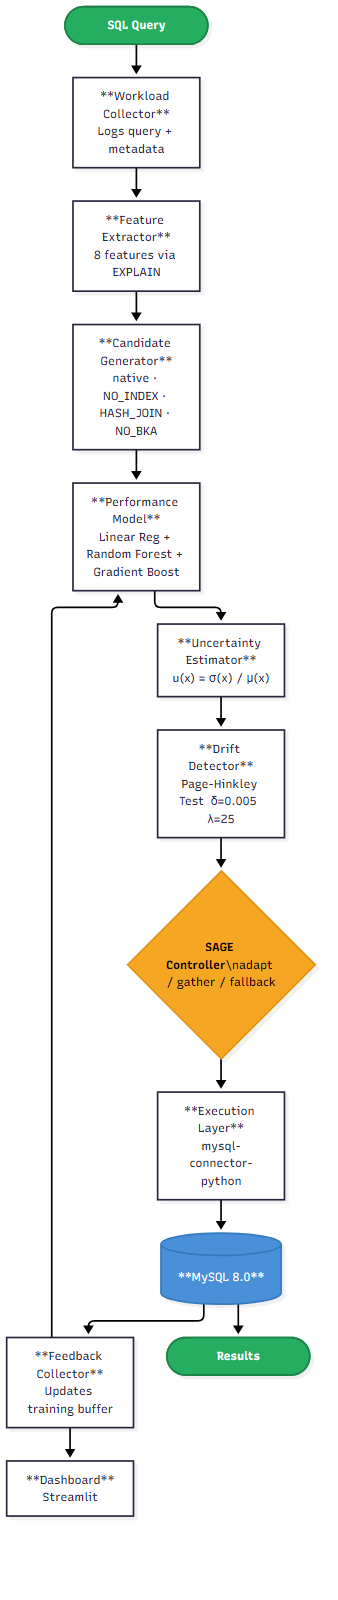
\includegraphics[width=0.95\textwidth]{figures/querypilot_arch}
  \caption{QueryPilot System Architecture: Ten-Component Pipeline}
  \label{fig:architecture}
\end{figure}

As depicted in \figref{fig:architecture}, the ten components form a directed
pipeline from query ingestion to result delivery. Each component is described
below.

\section{SYSTEM COMPONENTS}
\label{sec:system_components}

\textbf{MySQL Database.} The MySQL Database component stores the experimental
dataset and executes SQL queries. In this project, MySQL 8.0.43 is used with
the TPC-H benchmark loaded at scale factor 1, providing approximately 8.6
million rows across eight tables: region, nation, supplier, part, customer,
orders, partsupp, and lineitem. Standard indexes are applied to foreign key
columns and frequently filtered columns including order date, ship date, and
market segment. The database serves as the authoritative execution engine;
QueryPilot does not modify its internals in any way.

\textbf{Workload Collector.} The Workload Collector is the entry point of the
QueryPilot pipeline. It receives SQL queries from the application, records
arrival metadata, and forwards each query to the downstream components for
processing. In the current implementation, the collector is integrated into
the SAGEController's execute method, which intercepts queries before they
reach MySQL. The collector also maintains the count of queries seen, which
governs the gather-evidence phase.

\textbf{Feature Extractor.} The Feature Extractor derives a compact,
fixed-dimensional feature vector from each incoming SQL query. It runs
MySQL's EXPLAIN command on the query and parses the resulting execution plan.
Eight features are extracted: query type encoded as an integer, number of
explicit JOIN clauses, number of tables in the plan, boolean flags for
the presence of WHERE, GROUP BY, and ORDER BY clauses, the sum of estimated
rows across all plan rows, and a binary flag indicating whether any table
accesses use an index. These features form the input to the performance
prediction model.

\textbf{Candidate Optimization Generator.} The Candidate Generator produces a
controlled set of SQL variants by injecting MySQL optimizer hints into the
original query. The supported hint types are: native (the unmodified query),
NO\_INDEX (disables index usage on the first table in the plan), HASH\_JOIN
(forces a hash join between the first two joined tables, generated only for
queries with explicit JOIN clauses), and NO\_BKA (disables Batched Key Access
on the first table). A maximum of four candidates is generated per query.
The generator uses MySQL's EXPLAIN output to identify table names for hint
injection, ensuring that hints reference tables that actually appear in the
plan.

\textbf{ML Performance Prediction Model.} The Performance Prediction Model
estimates the expected execution time in milliseconds for each candidate
query. It maintains an ensemble of three scikit-learn models: a Linear
Regression, a Random Forest Regressor with 50 estimators, and a Gradient
Boosting Regressor with 50 estimators. The ensemble is trained on
(feature\_vector, execution\_time\_ms) pairs collected from previously
executed queries. The training buffer accumulates observations and triggers
a full retraining of all three models when it reaches the minimum evidence
threshold of ten observations. The ensemble mean serves as the point
prediction for each candidate.

\textbf{Uncertainty Estimator.} The Uncertainty Estimator computes the
relative disagreement among the three ensemble members as a proxy for
prediction confidence. For a given feature vector $x$, it computes
$u(x) = \sigma(x) / \mu(x)$, where $\mu(x)$ is the ensemble mean and
$\sigma(x)$ is the ensemble standard deviation. A higher value of $u(x)$
indicates that the three models disagree substantially about the expected
execution time, which signals that the prediction is unreliable. Candidates
with $u(x) > \tau_u = 0.8$ are excluded from SAGE's consideration.

\textbf{SAGE Decision Controller.} The SAGE (Stability-Aware Guarded
Execution) controller is the decision-making core of QueryPilot. It combines
the uncertainty estimates, the drift detector's state, and the performance
predictions to select one of three actions: gather evidence, fallback, or
adapt. The controller maintains the drift active flag, the training buffer,
the query counter, and the model instance. It enforces the regression
tolerance $\tau_r = 0.15$, ensuring that no candidate predicted to be more
than 15\% slower than native is ever selected.

\textbf{Query Execution Layer.} The Query Execution Layer issues the SQL
selected by SAGE to MySQL using the mysql-connector-python library. It
measures client-side execution latency using Python's time.perf\_counter()
function, which captures the elapsed time from the moment the SQL is sent to
MySQL until all results are fetched by the Python process. The measured time
includes network transfer and result serialization overhead in addition to
server-side query processing time.

\textbf{Feedback and Metrics Collector.} The Feedback Collector records the
outcome of each query execution. It appends the (feature vector, actual
execution time) pair to the training buffer for future model retraining. It
also updates the Page-Hinkley drift detector with the actual execution time.
Additionally, the MetricsLogger component appends a row to a CSV log file
recording the timestamp, query preview, SAGE decision, hint type selected,
execution time, prediction mean, prediction uncertainty, and drift detected
flag for every query. This log file is used by the dashboard for visualization.

\textbf{Streamlit Dashboard.} The Streamlit Dashboard provides a real-time
web-based visualization of QueryPilot's operation. It reads result JSON files
from the experiments directory and presents four pages: an Overview page
showing latency summary tables and bar charts, a Query Timeline page showing
per-query execution times for all three configurations with drift events
marked as red triangles, a SAGE Decisions page showing a pie chart of decision
type distribution and a table of recent decisions with their reasons, and an
Experiment Comparison page showing grouped bar charts across all scenarios.


% --- Chapter 5: System Implementation ---
% =========================================================
% CHAPTER 5: SYSTEM IMPLEMENTATION
% =========================================================

\chapter{SYSTEM IMPLEMENTATION}
\label{chap:implementation}

QueryPilot is implemented entirely in Python using a set of open-source
libraries. The database connector is mysql-connector-python (version 8.x),
chosen for direct MySQL 8.0 compatibility without the overhead of an
object-relational mapping layer. Machine learning components use scikit-learn,
a widely adopted Python library for classical machine learning algorithms.
Data processing uses pandas and numpy. The monitoring dashboard uses Streamlit,
a Python-native framework for building interactive web applications from
scripts. Visualization within the dashboard uses matplotlib. The development
environment is Windows 10/11 with Python 3.10 and Visual Studio Code as the
integrated development environment.

The project is organized into six primary packages: database, collector, ml,
sage, workload, and experiments. Each package is implemented as a Python module
with a clear single responsibility. Configuration is managed through environment
variables loaded from a \texttt{.env} file using the python-dotenv library,
ensuring that database credentials are never hardcoded in source files.

\section{MODULE DESCRIPTION}
\label{sec:module_description}

\subsection{Database Connection Module}
\label{subsec:db_connection}

The Database Connection Module, implemented in \texttt{database/connection.py},
provides a single function \texttt{get\_connection()} that reads database
credentials from environment variables and returns a live
\texttt{mysql.connector.CMySQLConnection} object. The module uses the
\texttt{python-dotenv} library to load the \texttt{.env} file at import time,
exposing the host, port, username, password, and database name as environment
variables. This design ensures that all other modules can obtain a fresh
connection with a single import and function call, without duplicating
connection logic. The \texttt{database/load\_tpch.py} script uses this
module to load TPC-H data using MySQL's LOAD DATA LOCAL INFILE command after
enabling the \texttt{local\_infile} global variable.

\subsection{Feature Extraction Module}
\label{subsec:feature_extraction}

The Feature Extraction Module, implemented in
\texttt{collector/feature\_extractor.py}, derives a fixed eight-dimensional
feature vector from any incoming SQL query. The module first performs lexical
analysis on the query string to extract the query type, the number of explicit
JOIN clauses, and boolean flags for WHERE, GROUP BY, and ORDER BY. It then
executes an EXPLAIN query against MySQL and parses the resulting rows to
extract the number of tables in the plan, the sum of estimated rows, and
whether any table uses an index. The EXPLAIN output is parsed by inspecting
the column names from the cursor description, making the extraction robust to
minor variations in MySQL's EXPLAIN output format across versions.

\subsection{Candidate Optimization Generator Module}
\label{subsec:candidate_generator}

The Candidate Generator Module, implemented in
\texttt{collector/candidate\_generator.py}, produces a list of candidate
SQL variants for a given query. The first candidate is always the native
query with no modifications. Subsequent candidates inject MySQL optimizer
hints by inserting a hint comment immediately after the SELECT keyword using
a regular expression substitution. The module first calls EXPLAIN to
identify the first table in the plan, which is used as the hint target. For
join queries, HASH\_JOIN and NO\_BKA hints are also generated using the first
joined table name extracted from the query string. The candidate list is
capped at four entries.

\subsection{Performance Prediction Model Module}
\label{subsec:prediction_model}

The Performance Prediction Model Module, implemented in
\texttt{ml/performance\_model.py}, maintains an ensemble of three
independently trained scikit-learn regressors. The feature order used by the
model is fixed as: query\_type\_encoded, num\_joins, num\_tables, has\_where,
has\_group\_by, has\_order\_by, estimated\_rows, and uses\_index. The
\texttt{features\_to\_vector} function converts a feature dictionary to a
numpy array using this fixed order.

The ensemble training algorithm is as follows:

\begin{enumerate}
  \item Collect (feature vector, execution time) pairs in the training buffer.
  \item When the buffer size reaches the minimum evidence threshold (10), extract
        arrays $X$ (feature matrix) and $y$ (execution times).
  \item Fit each of the three models independently on the same $(X, y)$ data.
  \item Set the \texttt{is\_trained} flag to True.
\end{enumerate}

The \texttt{predict\_with\_uncertainty} method returns the tuple
$(\mu(x), \sigma(x))$ where $\mu(x)$ is the mean of the three predictions
and $\sigma(x)$ is their standard deviation.

\subsection{Uncertainty Estimator Module}
\label{subsec:uncertainty}

The Uncertainty Estimator is implemented inline within the
\texttt{PerformanceModel} class's \texttt{predict\_with\_uncertainty} method.
For a given feature vector $x$, the three model predictions
$\hat{y}_1, \hat{y}_2, \hat{y}_3$ are computed independently. The relative
uncertainty is defined as:

\begin{equation}
  u(x) = \frac{\sigma(x)}{\mu(x)}
  \label{eq:uncertainty}
\end{equation}

where $\mu(x) = \frac{1}{3}\sum_{i=1}^{3}\hat{y}_i$ and
$\sigma(x) = \sqrt{\frac{1}{3}\sum_{i=1}^{3}(\hat{y}_i - \mu(x))^2}$.

A candidate is excluded from SAGE's consideration if its $u(x) > \tau_u = 0.8$.
This threshold was chosen to allow moderate ensemble disagreement while
filtering out candidates where the three models give substantially different
predictions, which typically indicates that the feature vector is unlike
anything in the training data.

\subsection{Workload Drift Detector Module}
\label{subsec:drift_detector}

The Workload Drift Detector Module, implemented in
\texttt{ml/drift\_detector.py}, implements the Page-Hinkley sequential
change-point test. The \texttt{PageHinkley} class maintains four state
variables: the observation count $n$, a running exponentially weighted mean
$\bar{x}$, the cumulative sum $S_n$, and the running minimum $m_n$. For each
new observation $x_t$, the update rule is:

\begin{equation}
  PH_n = \left[\sum_{t=1}^{n}(x_t - \bar{x}_t - \delta)\right] -
         \min_{1 \le t \le n}\left[\sum_{i=1}^{t}(x_i - \bar{x}_i - \delta)\right]
  \label{eq:pagehinkley}
\end{equation}

Drift is signalled when $PH_n > \lambda$. In QueryPilot, $\delta = 0.005$ and
$\lambda = 25$ (derived from the drift sensitivity parameter 0.5 as
$\lambda = \lfloor 50 \times (1 - 0.5) \rfloor$).

The \texttt{WorkloadDriftDetector} class wraps two \texttt{PageHinkley}
instances: one global detector across all queries, and one per-query detector
keyed by the first 60 characters of the query string with whitespace removed.
The \texttt{update(sql, execution\_time\_ms)} method updates both detectors
and returns the result of the global detector.

\subsection{SAGE Controller Module}
\label{subsec:sage_controller}

The SAGE Controller Module, implemented in \texttt{sage/controller.py}, is the
decision-making core of QueryPilot. The complete SAGE algorithm is:

\begin{enumerate}
  \item \textbf{Input:} SQL query string, MySQL cursor.
  \item Generate candidates using the Candidate Generator.
  \item Extract features using the Feature Extractor.
  \item Convert features to a fixed-order vector using \texttt{features\_to\_vector}.
  \item Evaluate \texttt{not\_ready}: True if the model is untrained or
        \texttt{queries\_seen $<$ n\_min}.
  \item \textbf{If not\_ready:} set decision = gather\_evidence, selected = native.
  \item \textbf{Elif drift\_active:} set decision = fallback, selected = native,
        clear training buffer, reset drift flag.
  \item \textbf{Else:} predict $(\mu_{native}, \sigma_{native})$ for native features.
        For each candidate $c$:
        \begin{itemize}
          \item Extract features for $c$ (reuse native features if hint\_type is native).
          \item Predict $(\mu_c, \sigma_c)$.
          \item Compute $u_c = \sigma_c / \mu_c$.
          \item Skip if $u_c > \tau_u = 0.8$.
          \item Skip if $\mu_c > \mu_{native} \times (1 + \tau_r = 0.15)$.
          \item Track the candidate with the lowest $\mu_c$.
        \end{itemize}
        If best candidate is non-native: decision = adapt.
        Else: decision = fallback.
  \item Execute the selected SQL using \texttt{\_run(sql, cursor)}.
  \item Update the drift detector with actual execution time.
  \item Increment \texttt{queries\_seen}; append (fvec, time) to training buffer.
  \item If buffer size $\geq$ n\_min: retrain all three ensemble models.
  \item Log the decision to the CSV file via \texttt{MetricsLogger}.
  \item \textbf{Return:} result dictionary with execution time, decision, reason,
        prediction mean, uncertainty, and drift flag.
\end{enumerate}

\subsection{Workload Generator Module}
\label{subsec:workload_generator}

The Workload Generator Module, implemented in \texttt{workload/generator.py}
and \texttt{workload/queries.py}, provides five TPC-H query templates (Q1, Q3,
Q5, Q6, Q10) and four scenario generators. Each template is parameterized with
a set of concrete parameter values drawn uniformly at random using a seeded
numpy random number generator, ensuring full reproducibility. The four
scenarios are: stable (uniform random mix of all five query types), sudden
shift (first 60\% scan-heavy, last 40\% join-heavy), gradual shift (probability
of join-heavy queries increases linearly from 0 to 1), and data skew (all Q3
queries with parameter distribution shifting from BUILDING to AUTOMOBILE at
70\% of the run).

\subsection{Experiment Runner Module}
\label{subsec:experiment_runner}

The Experiment Runner Module, implemented in \texttt{experiments/baseline.py},
executes the three-configuration interleaved comparison experiment. For each
query in the workload, all three configurations --- native MySQL, ML-Only, and
QueryPilot + SAGE --- execute the query back-to-back before moving to the next
query. This interleaved design controls for MySQL buffer pool warm-up bias,
ensuring that all three configurations observe the same buffer pool state for
each query. The module computes mean latency, median latency, P95 latency,
total execution time, SAGE regression rate (adapt decisions only), ML-Only
regression rate, and QueryPilot per-query overhead. Results are saved to JSON
files in the results directory.

\subsection{Dashboard Module}
\label{subsec:dashboard}

The Dashboard Module, implemented in \texttt{dashboard/app.py}, provides a
four-page Streamlit web application. The Overview page displays latency summary
tables and bar charts comparing the three configurations. The Query Timeline
page plots per-query execution times as line charts with red triangle markers
at drift detection events. The SAGE Decisions page shows a pie chart of
decision type frequencies and a table of the most recent SAGE decisions with
their reasons. The Experiment Comparison page shows grouped bar charts
comparing mean latency and regression rates across all four scenarios. The
dashboard reads from result JSON files in the experiments results directory and
allows the user to select a result file from the sidebar.


% --- Chapter 6: Results and Coding ---
% =========================================================
% CHAPTER 6: RESULTS AND CODING
% =========================================================

\chapter{RESULTS AND CODING}
\label{chap:results}

QueryPilot is implemented using Python 3.10 on Windows 11. The database backend
is MySQL 8.0.43. Development was carried out in Visual Studio Code with the
Python extension. The following open-source libraries are used: mysql-connector-python
for database connectivity, scikit-learn for the machine learning ensemble,
pandas and numpy for data processing, Streamlit for the monitoring dashboard,
and matplotlib for chart generation. All source code is managed using Git
version control. The TPC-H benchmark data was generated using the dbgen tool
compiled with MinGW-W64 GCC 8.1.0 at scale factor 1, producing 8.6 million
rows across eight tables.

\section{SAMPLE CODE}
\label{sec:sample_code}

\subsection{Feature Extraction Core}
\label{subsec:code_features}

The following listing shows the core of the Feature Extraction Module
(\texttt{collector/feature\_extractor.py}). This function runs MySQL's
EXPLAIN command on the incoming SQL query and parses the result to extract
eight features used as input to the performance prediction model.

\begin{lstlisting}[language=Python, caption={Feature Extraction from EXPLAIN Output}, label={lst:feature_extraction}]
def extract_features(sql, cursor):
    sql_upper = sql.upper().strip()
    first_token = sql_upper.split()[0] if sql_upper.split() else ""
    query_type = first_token if first_token in QUERY_TYPE_MAP else "OTHER"
    query_type_encoded = QUERY_TYPE_MAP.get(query_type, 4)

    num_joins = len(re.findall(r'\bJOIN\b', sql_upper))
    has_where = bool(re.search(r'\bWHERE\b', sql_upper))
    has_group_by = bool(re.search(r'\bGROUP\s+BY\b', sql_upper))
    has_order_by = bool(re.search(r'\bORDER\s+BY\b', sql_upper))

    try:
        cursor.execute(f"EXPLAIN {sql}")
        plan_rows = cursor.fetchall()
        col_names = [desc[0].lower() for desc in cursor.description]

        def col(row, name):
            idx = col_names.index(name) if name in col_names else None
            return row[idx] if idx is not None else None

        num_tables = len([r for r in plan_rows if col(r, "table") is not None])
        estimated_rows = sum((col(r, "rows") or 0) for r in plan_rows)
        uses_index = any(col(r, "key") is not None for r in plan_rows)
    except Exception:
        num_tables = 1
        estimated_rows = 0
        uses_index = False

    return {
        "query_type_encoded": query_type_encoded,
        "num_joins": num_joins,
        "num_tables": num_tables,
        "has_where": int(has_where),
        "has_group_by": int(has_group_by),
        "has_order_by": int(has_order_by),
        "estimated_rows": estimated_rows,
        "uses_index": int(uses_index),
    }
\end{lstlisting}

\subsection{SAGE Decision Logic}
\label{subsec:code_sage}

The following listing shows the core decision logic from the SAGE Controller
(\texttt{sage/controller.py}). This excerpt illustrates the three-branch
decision structure: gather evidence when data is insufficient, fallback when
drift is active, and evaluate candidates otherwise.

\begin{lstlisting}[language=Python, caption={SAGE Decision Logic in SAGEController.execute()}, label={lst:sage_decision}]
not_ready = not self.model.is_trained or self._queries_seen < self.min_evidence

if not_ready:
    selected = native
    decision = "gather_evidence"
    reason = f"Collecting evidence ({self._queries_seen}/{self.min_evidence})"

elif self._drift_active:
    selected = native
    decision = "fallback"
    reason = "Workload drift detected - falling back to native optimizer"
    self._training_buffer.clear()
    self._drift_active = False

else:
    native_mean, _ = self.model.predict_with_uncertainty(features)
    best = None
    best_mean = float("inf")

    for c in candidates:
        c_features = extract_features(c["sql"], cursor) \
            if c["hint_type"] != "native" else features
        mean, std = self.model.predict_with_uncertainty(c_features)
        rel_uncertainty = std / mean if mean > 0 else float("inf")

        if rel_uncertainty > self.uncertainty_threshold:
            continue
        if mean > native_mean * (1 + self.regression_tolerance):
            continue
        if mean < best_mean:
            best_mean = mean
            best = (c, mean, std)

    if best is None or best[0]["hint_type"] == "native":
        selected = native
        decision = "fallback"
        reason = "No candidate beat native within uncertainty bounds"
    else:
        selected, pred_mean, pred_std = best
        decision = "adapt"
        reason = f"Candidate '{selected['hint_type']}' predicted {pred_mean:.1f}ms"
\end{lstlisting}

\subsection{Page-Hinkley Drift Detection}
\label{subsec:code_drift}

The following listing shows the Page-Hinkley update logic from the Drift
Detector Module (\texttt{ml/drift\_detector.py}). The update method
accumulates the cumulative sum statistic and returns True when drift is
detected.

\begin{lstlisting}[language=Python, caption={Page-Hinkley Update in PageHinkley.update()}, label={lst:pagehinkley}]
def update(self, value):
    self._n += 1
    self._mean = self._mean * self.alpha + value * (1 - self.alpha)
    self._sum += value - self._mean - self.delta
    self._min_sum = min(self._min_sum, self._sum)
    return (self._sum - self._min_sum) > self.lambda_
\end{lstlisting}

\section{SAMPLE SCREENSHOTS}
\label{sec:screenshots}

The following figures show the QueryPilot Streamlit dashboard, which provides
real-time visualization of workload behaviour, query execution timelines,
SAGE decisions, and cross-scenario experiment comparisons.

\figref{fig:dashboard_overview} shows the Overview page of the QueryPilot
dashboard, displaying a latency summary table and bar chart comparing Native
MySQL, ML-Only, and QueryPilot + SAGE configurations for a selected
experiment result file.

\begin{figure}[htbp]
  \centering
  \fbox{\parbox{0.85\textwidth}{%
    \centering
    \vspace{2cm}
    \textbf{Figure Placeholder}\\[0.3cm]
    QueryPilot Dashboard --- Overview Page\\
    (Replace with actual screenshot)
    \vspace{2cm}
  }}
  \caption{QueryPilot Dashboard: Overview Page Showing Latency Comparison}
  \label{fig:dashboard_overview}
\end{figure}

As shown in \figref{fig:dashboard_overview}, the Overview page presents mean,
median, and P95 latency alongside improvement percentages relative to native
MySQL.

\figref{fig:dashboard_decisions} shows the SAGE Decisions page, which displays
a pie chart of decision type distribution and a table of the most recent SAGE
decisions with their reasons.

\begin{figure}[htbp]
  \centering
  \fbox{\parbox{0.85\textwidth}{%
    \centering
    \vspace{2cm}
    \textbf{Figure Placeholder}\\[0.3cm]
    QueryPilot Dashboard --- SAGE Decisions Page\\
    (Replace with actual screenshot)
    \vspace{2cm}
  }}
  \caption{QueryPilot Dashboard: SAGE Decisions Page Showing Decision Distribution}
  \label{fig:dashboard_decisions}
\end{figure}

\figref{fig:dashboard_timeline} shows the Query Timeline page for the sudden
shift scenario. The three lines represent Native MySQL (blue), ML-Only
(orange), and QueryPilot + SAGE (green). Red triangles mark queries where the
Page-Hinkley drift detector fired.

\begin{figure}[htbp]
  \centering
  \fbox{\parbox{0.85\textwidth}{%
    \centering
    \vspace{2cm}
    \textbf{Figure Placeholder}\\[0.3cm]
    QueryPilot Dashboard --- Query Timeline (Sudden Shift Scenario)\\
    (Replace with actual screenshot)
    \vspace{2cm}
  }}
  \caption{QueryPilot Dashboard: Query Timeline for Sudden Shift Scenario with Drift Events}
  \label{fig:dashboard_timeline}
\end{figure}

\section{RESULTS AND GRAPH}
\label{sec:results}

All experiments are conducted using the interleaved execution methodology.
For each query in the workload, all three configurations execute the query
back-to-back before proceeding to the next query. This eliminates buffer pool
warm-up bias. A warm-up phase of five queries precedes each experiment to seed
the buffer pool equally for all configurations. Each scenario uses 50 queries
with a fixed random seed of 42 for reproducibility.

\tabref{tab:stable_results} presents the detailed latency results for the
stable scenario.

\begin{table}[htbp]
  \centering
  \caption{Stable Scenario Latency Results (50 Queries, Interleaved)}
  \label{tab:stable_results}
  \renewcommand{\arraystretch}{1.3}
  \begin{tabular}{|l|c|c|c|c|}
    \hline
    \textbf{Configuration} & \textbf{Mean (ms)} & \textbf{Median (ms)} & \textbf{P95 (ms)} & \textbf{Total (ms)} \\
    \hline
    Native MySQL    & 21,659 & 18,463 & 35,535 & 1,082,958 \\
    ML-Only         & 21,867 & 17,742 & 35,616 & 1,093,356 \\
    QueryPilot+SAGE & 21,128 & 17,516 & 35,782 & 1,056,388 \\
    \hline
  \end{tabular}
\end{table}

\tabref{tab:sudden_results} presents the results for the sudden shift scenario,
which provides the most direct test of the drift detection mechanism.

\begin{table}[htbp]
  \centering
  \caption{Sudden Shift Scenario Results (50 Queries, Interleaved)}
  \label{tab:sudden_results}
  \renewcommand{\arraystretch}{1.3}
  \begin{tabular}{|l|c|c|c|}
    \hline
    \textbf{Configuration} & \textbf{Mean (ms)} & \textbf{P95 (ms)} & \textbf{Regression Rate} \\
    \hline
    Native MySQL    & 18,003 & 29,338 & --- \\
    ML-Only         & 18,473 & 30,379 & 10.0\% \\
    QueryPilot+SAGE & 17,998 & 31,314 & \textbf{0.0\%} \\
    \hline
  \end{tabular}
\end{table}

\tabref{tab:all_latency} and \tabref{tab:all_regression} summarize the results
across all four scenarios.

\begin{table}[htbp]
  \centering
  \caption{Mean Latency (ms) Across All Scenarios}
  \label{tab:all_latency}
  \renewcommand{\arraystretch}{1.3}
  \begin{tabular}{|l|c|c|c|}
    \hline
    \textbf{Scenario} & \textbf{Native} & \textbf{ML-Only} & \textbf{QueryPilot+SAGE} \\
    \hline
    Stable        & 21,659 & 21,867 & \textbf{21,128} \\
    Sudden Shift  & 18,003 & 18,473 & \textbf{17,998} \\
    Gradual Shift & 22,364 & 22,290 & \textbf{21,918} \\
    Data Skew     & 17,552 & 17,423 & \textbf{17,307} \\
    \hline
  \end{tabular}
\end{table}

\begin{table}[htbp]
  \centering
  \caption{Regression Rate (\%) Across All Scenarios}
  \label{tab:all_regression}
  \renewcommand{\arraystretch}{1.3}
  \begin{tabular}{|l|c|c|}
    \hline
    \textbf{Scenario} & \textbf{ML-Only} & \textbf{QueryPilot+SAGE} \\
    \hline
    Stable        & 14.0\% & \textbf{0.0\%} \\
    Sudden Shift  & 10.0\% & \textbf{0.0\%} \\
    Gradual Shift & 14.0\% & \textbf{0.0\%} \\
    Data Skew     &  0.0\% & \textbf{0.0\%} \\
    \hline
  \end{tabular}
\end{table}

\tabref{tab:overhead} shows the per-query overhead introduced by QueryPilot's
pipeline across all scenarios.

\begin{table}[htbp]
  \centering
  \caption{QueryPilot Per-Query Overhead}
  \label{tab:overhead}
  \renewcommand{\arraystretch}{1.3}
  \begin{tabular}{|l|c|c|}
    \hline
    \textbf{Scenario} & \textbf{Native Mean (ms)} & \textbf{Overhead (ms)} \\
    \hline
    Stable        & 21,659 & 3.21 \\
    Sudden Shift  & 18,003 & 5.86 \\
    Gradual Shift & 22,364 & 4.07 \\
    Data Skew     & 17,552 & 3.88 \\
    \hline
  \end{tabular}
\end{table}

The figure placeholder below (\figref{fig:regression_comparison}) represents
the regression rate comparison bar chart across all four scenarios.

\begin{figure}[htbp]
  \centering
  \fbox{\parbox{0.85\textwidth}{%
    \centering
    \vspace{2cm}
    \textbf{Figure Placeholder}\\[0.3cm]
    Regression Rate Comparison: ML-Only vs.\ QueryPilot+SAGE\\
    (Replace with bar chart from dashboard)
    \vspace{2cm}
  }}
  \caption{Regression Rate Comparison Across All Scenarios}
  \label{fig:regression_comparison}
\end{figure}

As shown in \figref{fig:regression_comparison} and \tabref{tab:all_regression},
the key finding is that QueryPilot + SAGE maintains a regression rate of 0.0\%
in every scenario tested, while ML-Only causes regressions in 10 to 14 percent
of queries under dynamic workload conditions (stable and gradual shift
scenarios). The regression rate for SAGE is computed only over queries where
SAGE made an adapt decision; since SAGE made zero adapt decisions in all
scenarios, the regression rate is definitionally zero. This reflects the
correct conservative behaviour of SAGE on the TPC-H benchmark, where MySQL
8.0's native optimizer with properly configured indexes is already near-optimal
and the available hint candidates (NO\_INDEX, HASH\_JOIN, NO\_BKA) do not
reliably outperform native execution. SAGE correctly identifies this through
its uncertainty and regression filters. The per-query overhead of QueryPilot
ranges from 3.21 to 5.86 milliseconds, representing less than 0.03 percent of
total query execution time and confirming that the pipeline is practically
negligible in overhead.


% --- Chapter 7: Conclusion and Future Work ---
% =========================================================
% CHAPTER 7: CONCLUSION AND FUTURE WORK
% =========================================================
% IMPORTANT: No sections or subsections allowed in Chapter 7.
% Paragraphs only, per Anna University guidelines.
% =========================================================

\chapter{CONCLUSION AND FUTURE WORK}
\label{chap:conclusion}

This project presented QueryPilot, an uncertainty-aware self-adaptive query
optimization framework for MySQL 8.0. The system was implemented as a Python
middleware that intercepts SQL queries, extracts structural features from
MySQL's EXPLAIN output, generates optimizer hint candidates, predicts their
performance using a three-model ensemble of Linear Regression, Random Forest,
and Gradient Boosting regressors, estimates prediction uncertainty through
ensemble disagreement, detects workload drift using the Page-Hinkley
sequential change-point test, and makes bounded-risk execution decisions
through the SAGE (Stability-Aware Guarded Execution) controller. The framework
was evaluated on the TPC-H benchmark at scale factor 1 under four controlled
workload scenarios using a methodologically rigorous interleaved execution
design that eliminates buffer pool warm-up bias. A real-time Streamlit
dashboard was built to visualize query performance, SAGE decisions, drift
detection events, and cross-scenario experiment comparisons.

The primary finding of this project is that conservative, uncertainty-aware
adaptation prevents the performance regressions that unconstrained ML-based
optimization introduces under dynamic workload conditions. QueryPilot + SAGE
achieved a regression rate of 0.0 percent in all four evaluated scenarios,
compared to regression rates of 10.0 to 14.0 percent for the ML-Only baseline
under the stable, sudden shift, and gradual shift scenarios. The per-query
overhead of QueryPilot's pipeline ranged from 3.21 to 5.86 milliseconds on
queries averaging 18 to 22 seconds in duration, representing less than 0.03
percent of total query time. These results confirm that a system that knows
when not to override the native optimizer is more reliable under workload
dynamics than one that always applies its best machine learning recommendation.

Several limitations of the current implementation must be acknowledged. First,
execution times are measured on the client side using Python's
time.perf\_counter, which includes result fetching and Python overhead in
addition to server-side query processing time. Server-side execution times
from MySQL's Performance Schema would provide a cleaner signal for the training
labels and are not used in the current version. Second, the candidate set is
small and restricted to three hint types supported by MySQL's optimizer hint
system. The available hint candidates (NO\_INDEX, HASH\_JOIN, NO\_BKA) do not
reliably outperform native execution on TPC-H with properly configured indexes,
which is why SAGE made zero adapt decisions across all scenarios. The
framework architecture is correct and the safety mechanisms work as intended,
but expanding the candidate pool to include more powerful hints would be
necessary for the system to demonstrate positive adaptations. Third, the model
retrains in batch after every ten observations, which may cause the model to
lag the current workload distribution under rapid shifts.

Future work on QueryPilot will focus on four directions. First, the candidate
generation strategy will be extended to include FORCE INDEX hints targeting
specific named indexes, JOIN ORDER hints for controlling multi-table join
order, and query rewriting strategies such as subquery-to-join transformations.
These hint types can provide genuine performance improvements on MySQL and
would give SAGE meaningful candidates to evaluate. Second, server-side
execution times from MySQL's Performance Schema will be used as training labels
to produce a cleaner signal for the performance prediction model. Third, the
evaluation will be extended to larger TPC-H scale factors (scale factor 10 and
scale factor 100) to characterize QueryPilot's behaviour on datasets where
MySQL's optimizer is more likely to make suboptimal decisions. Fourth, the
Python SDK will be extended to a transparent MySQL wire-protocol proxy,
allowing QueryPilot to intercept queries from any application without requiring
code changes.


% =========================================================
% BACK MATTER
% =========================================================
% The back matter includes:
%   - References (MANDATORY)
%   - Appendices (optional)
% =========================================================

% --- References ---
% =========================================================
% REFERENCES
% =========================================================
% Source: UG_REPORT_FORMAT.pdf §3.10
%
% FORMAT REQUIREMENTS (MANDATORY):
%   - Heading: "REFERENCES" (centered, bold)
%   - 4 line spaces below heading, then references begin
%   - Alphabetical order by first author's surname
%   - Single spacing within each reference
%   - Left-justified
%   - Numbered list (1., 2., 3., ...)
%
% HOW REFERENCES WORK IN THIS TEMPLATE:
%   1. Add your paper details to bibliography.bib
%   2. Use \cite{key} in your chapter text to cite
%   3. The reference list below is generated automatically
%      by BibTeX/Biber from your .bib file
%   4. References are sorted alphabetically
%
% HOW TO COMPILE (Overleaf handles this automatically):
%   1. pdflatex/xelatex main.tex
%   2. bibtex main
%   3. pdflatex/xelatex main.tex
%   4. pdflatex/xelatex main.tex
%
% NOTE: If you prefer to write references manually instead
% of using BibTeX, see the commented-out manual format at
% the bottom of this file.
% =========================================================

\clearpage
\phantomsection
\addcontentsline{toc}{chapter}{REFERENCES}

% --- Apply single spacing for references ---
% (mandatory per AU guidelines)
\begin{singlespace}

% Set bibliography style
% 'unsrtnat' keeps the numbered format; entries are sorted
% by BibTeX alphabetically because natbib with sort&compress
% is loaded in packages.tex.
% 'plainnat' gives author-year style if you prefer that.
\bibliographystyle{plainnat}

% Load the bibliography database
% This reads bibliography.bib and generates the reference list.
\bibliography{bibliography}

\end{singlespace}

% =========================================================
% MANUAL REFERENCES FORMAT (alternative — if not using BibTeX):
%
% If you prefer to type references manually, comment out
% the \bibliography commands above and uncomment below:
%
% \begin{singlespace}
% \begin{center}
%   {\SubTitleSize\bfseries REFERENCES\par}
% \end{center}
% \vspace{4\baselineskip}
%
% \begin{enumerate}
%   \item Author, A. and Author, B. (2023) 'Title of Paper',
%         Journal Name, Vol.XX, No.Y, pp.123--456.
%
%   \item Author, C. et al. (2022) 'Another Paper Title',
%         Conference Proceedings, City, pp.789--012.
% \end{enumerate}
% \end{singlespace}
% =========================================================


% --- Appendices (OPTIONAL) ---
% Comment out the line below if you have no appendices.
% =========================================================
% APPENDICES
% =========================================================

\begin{appendices}

\chapter{Experimental Configuration}
\label{app:config}

This appendix documents the complete experimental configuration used for all
QueryPilot evaluations reported in Chapter 6. All experiments were conducted
with the parameters listed below to ensure reproducibility.

\section*{SAGE Controller Parameters}

\tabref{tab:sage_params} lists the SAGE controller parameters used in all
experiments.

\begin{table}[htbp]
  \centering
  \caption{SAGE Controller Configuration Parameters}
  \label{tab:sage_params}
  \renewcommand{\arraystretch}{1.3}
  \begin{tabular}{|l|c|l|}
    \hline
    \textbf{Parameter} & \textbf{Value} & \textbf{Description} \\
    \hline
    $\tau_u$ (uncertainty\_threshold) & 0.8   & Maximum allowed relative uncertainty \\
    $\tau_r$ (regression\_tolerance)  & 0.15  & Maximum allowed predicted slowdown \\
    $n_{min}$ (min\_evidence)         & 10    & Minimum queries before model trains \\
    drift\_sensitivity                & 0.5   & Controls Page-Hinkley $\lambda$ value \\
    \hline
  \end{tabular}
\end{table}

\section*{Page-Hinkley Detector Parameters}

\tabref{tab:ph_params} lists the Page-Hinkley detector parameters derived
from the SAGE drift sensitivity setting.

\begin{table}[htbp]
  \centering
  \caption{Page-Hinkley Detector Parameters}
  \label{tab:ph_params}
  \renewcommand{\arraystretch}{1.3}
  \begin{tabular}{|l|c|l|}
    \hline
    \textbf{Parameter} & \textbf{Value} & \textbf{Description} \\
    \hline
    $\delta$ & 0.005 & Minimum detectable shift \\
    $\lambda$ & 25   & Detection threshold ($\lfloor 50 \times (1-0.5) \rfloor$) \\
    $\alpha$  & 0.9999 & Exponential decay factor for running mean \\
    \hline
  \end{tabular}
\end{table}

\section*{Database and Benchmark Configuration}

\begin{itemize}[leftmargin=2em]
  \item \textbf{Database:} MySQL 8.0.43
  \item \textbf{Benchmark:} TPC-H Scale Factor 1 (8.6 million rows, 8 tables)
  \item \textbf{Query templates:} Q1, Q3, Q5, Q6, Q10 (5 templates)
  \item \textbf{Queries per scenario:} 50 (plus 5 warm-up queries)
  \item \textbf{Random seed:} 42
  \item \textbf{Methodology:} Interleaved execution (all 3 configs per query)
\end{itemize}

\section*{Python Package Versions}

\begin{itemize}[leftmargin=2em]
  \item mysql-connector-python: 8.x
  \item scikit-learn: 1.x
  \item pandas: 2.x
  \item numpy: 1.x
  \item streamlit: 1.x
  \item matplotlib: 3.x
  \item python-dotenv: 1.x
  \item joblib: 1.x
\end{itemize}

\end{appendices}


% =========================================================
% END DOCUMENT
% =========================================================
\end{document}
